% !TeX program = xelatex
% !BIB program = biber
% !TeX root = SWJTU_Bachelor_Thesis.tex
% chktex-file 1
% chktex-file 44

%%% ======================= 导言 ======================= %%%
\documentclass[
  autoindent=true,
  fontset=none,
  linespread=1.5,
  UTF8,
  openany,
  twoside,
  zihao=-4
]{ctexbook}
\usepackage[major=计算机科学与技术]{style/swjtu}
\usepackage{array}

\begin{document}
%%% ======================= 前置 ======================= %%%
%%% ----------------------- 封面 ----------------------- %%%
\begin{titlepage}
  \thispagestyle{empty}
  \singlespacing

  \begin{center}
    \vspace*{0.3cm}
    
\includegraphics[width=0.66\textwidth]{images/logo.png}\par
    \vspace{1.4cm}

    {\songti\zihao{0}{\makebox[0.58\textwidth][c]{\strut 零售物品智能识别系统}}}\par
    \vspace{0.9cm}
    {\songti\zihao{2}{\makebox[0.58\textwidth][c]{\strut 基于yolov8的零售物品智能识别系统}}}\par
  \end{center}

  \vspace{1.2cm}
  \begin{center}
    \renewcommand{\arraystretch}{1.7}
    \begin{tabular}{@{}l p{9.0cm}@{}}
      {\heiti\zihao{3}设计人员：}
                             & \underline{\makebox[9.0cm][c]{\zihao{3}2023112594——陶秋源}}      \\
                             & \underline{\makebox[9.0cm][c]{\zihao{3}2023112476——马熙翔}}      \\
                             & \underline{\makebox[9.0cm][c]{\zihao{3}2023112579——王昊宇}}      \\
                             & \underline{\makebox[9.0cm][c]{\zihao{3}2023112567——程\quad 赞}} \\
      {\heiti\zihao{3}指导教师：} & \underline{\makebox[9.0cm][c]{\zihao{3}李威、殷成风}}               \\
    \end{tabular}
  \end{center}

  \vfill

  \begin{center}
    \renewcommand{\arraystretch}{1.30}
    \setlength{\tabcolsep}{5pt}
    \begin{tabular}{|
      >{\centering\arraybackslash}m{4.0cm}|
      >{\raggedright\arraybackslash}m{3.8cm}|
      >{\centering\arraybackslash}m{4.4cm}|}
      \hline
      \cellcolor[RGB]{187,224,227}\songti                      & \cellcolor[RGB]{187,224,227}\songti 文件标识  & \cellcolor[RGB]{187,224,227}\songti 1.0        \\
      \arrayrulecolor[RGB]{187,224,227}\hline
      \arrayrulecolor{black}\cline{2-3}
      \cellcolor[RGB]{187,224,227}\songti 文件状态：                & \cellcolor[RGB]{231,243,244}\songti 当前版本  & \cellcolor[RGB]{231,243,244}\songti V1.0       \\
      \arrayrulecolor[RGB]{187,224,227}\hline
      \arrayrulecolor{black}\cline{2-3}
      \cellcolor[RGB]{187,224,227}\songti [\(\checkmark\)] 草\hspace{1.5em} 稿 & \cellcolor[RGB]{243,249,250}\songti 拟 稿 人 & \cellcolor[RGB]{243,249,250}\songti 王昊宇、程赞     \\
      \arrayrulecolor[RGB]{187,224,227}\hline
      \arrayrulecolor{black}\cline{2-3}
      \cellcolor[RGB]{187,224,227}\songti [\ \ ] 正式发布          & \cellcolor[RGB]{231,243,244}\songti 拟稿日期  & \cellcolor[RGB]{231,243,244}\songti 2026年4月23日 \\
      \arrayrulecolor[RGB]{187,224,227}\hline
      \arrayrulecolor{black}\cline{2-3}
      \cellcolor[RGB]{187,224,227}\songti [\ \ ] 正在修改          & \cellcolor[RGB]{243,249,250}\songti 审 核 人 & \cellcolor[RGB]{243,249,250}\songti 陶秋源、马熙翔    \\
      \arrayrulecolor[RGB]{187,224,227}\hline
      \arrayrulecolor{black}\cline{2-3}
      \cellcolor[RGB]{187,224,227}\songti                      & \cellcolor[RGB]{231,243,244}\songti 审核日期  & \cellcolor[RGB]{231,243,244}\songti 2026年4月26日 \\ \hline
    \end{tabular}
  \end{center}
\end{titlepage}

%%% --------------------- 编写说明 --------------------- %%%
% \begin{emptyPage}
%   \singlespacing

%   \begin{center}
%     \vspace*{1.1cm}
%     {\heiti\zihao{2}编写说明\par}
%   \end{center}

%   \vspace{1.2cm}
%   {\songti\zihao{-4}
%     \noindent 标题：软件需求规格说明书（xxxx子系统）\par
%     \vspace{0.9\baselineskip}
%     \noindent 类别：文档\par
%     \vspace{0.9\baselineskip}
%     \noindent 存放位置：项目文档\textbackslash{}02、项目需求项-x-xxxxxx-软件需求规格说明书\par
%     \noindent \hspace*{3.2em}（xxxx子系统）-V1.0.1.doc\par
%     \vspace{0.9\baselineskip}
%     \noindent 编辑软件：Microsoft Word 2023 中文版\par
%   }

%   \vspace{1.2\baselineskip}
%   {\songti\zihao{-4}\noindent 版本历史：\par}
%   \vspace{0.4\baselineskip}
%   \renewcommand{\arraystretch}{1.25}
%   \setlength{\tabcolsep}{4pt}
%   \begin{tabularx}{\linewidth}{|
%     >{\centering\arraybackslash}m{1.7cm}|
%     >{\centering\arraybackslash}m{1.8cm}|
%     >{\centering\arraybackslash}m{2.0cm}|
%     >{\centering\arraybackslash}X|}
%     \hline
%     \heiti 版本 & \heiti 作者 & \heiti 日期 & \heiti 备注 \\ \hline
%     V1.0.1 &  &  &  \\ \hline
%      &  &  &  \\ \hline
%      &  &  &  \\ \hline
%      &  &  &  \\ \hline
%      &  &  &  \\ \hline
%      &  &  &  \\ \hline
%   \end{tabularx}

%   \vspace{1.2\baselineskip}
%   {\songti\zihao{-4}\noindent 完成情况分工：\par}
%   \vspace{0.4\baselineskip}
%   \begin{tabularx}{\linewidth}{|
%     >{\centering\arraybackslash}m{1.7cm}|
%     >{\centering\arraybackslash}m{1.8cm}|
%     >{\centering\arraybackslash}m{2.0cm}|
%     >{\centering\arraybackslash}X|}
%     \hline
%     \heiti 学号 & \heiti 姓名 & \heiti 工作量 & \heiti 完成工作内容 \\ \hline
%      &  & 百分比 &  \\ \hline
%      &  &  &  \\ \hline
%      &  &  &  \\ \hline
%      &  &  &  \\ \hline
%      &  &  &  \\ \hline
%      &  &  &  \\ \hline
%   \end{tabularx}
% \end{emptyPage}

%%% ======================= 目录 ======================= %%%
\swjtuTableOfContents

%%% ======================= 正文 ======================= %%%
% \include{chapters/introduction}
\swjtuChapter{软件需求规格说明书}

% 去掉章节前缀，使用 1 / 1.1 / 1.1.1 的编号体系
\setcounter{section}{0}
\renewcommand{\thesection}{\arabic{section}}
\renewcommand{\thesubsection}{\thesection.\arabic{subsection}}
\renewcommand{\thesubsubsection}{\thesubsection.\arabic{subsubsection}}

\section{概述}

\subsection{背景}
随着人工智能（AI）与计算机视觉（CV）技术的飞速发展，传统零售行业的数字化转型已成为必然趋势。传统商超主要依赖人工盘点与条码扫描结算，存在结算高峰期拥堵、用户寻物困难、库存数据更新滞后等显著痛点。本项目旨在利用先进的深度学习目标检测算法，结合 Web 全栈技术，开发一套低成本、高效率的“零售物品智能识别系统”，以期实现商超场景下的视觉导购、无感自助结算及供应链自动预警，全面提升运营效率与顾客体验。

\subsection{编写目标}
本文档旨在全面、准确地描述“零售物品智能识别系统”的功能性需求与非功能性需求。本文档将作为项目架构设计、代码编码、软件测试以及最终期末验收的核心基准文件，确保开发人员、测试人员与系统干系人对系统边界和业务逻辑达成一致理解。

\subsection{相关术语定义}
\begin{itemize}[leftmargin=2em]
  \item CV (Computer Vision)：计算机视觉，一门研究如何使机器“看”的科学，本系统中主要用于处理摄像头视频流。
  \item YOLO (You Only Look Once)：一种端到端的实时目标检测（Object Detection）算法，本系统采用其轻量级版本实现商品的毫秒级定位与分类。
  \item B/S 架构（Browser/Server）：浏览器/服务器模式，本系统的主要网络架构，用户只需通过浏览器即可访问系统，无需安装客户端。
  \item FastAPI：一个现代、快速（高性能）的 Python Web 框架，基于标准 Python 类型提示，用于构建本系统的后端 API 接口。
  \item ORM (Object-Relational Mapping)：对象关系映射，本系统通过 SQLAlchemy 实现面向对象的数据库操作，避免直接拼接 SQL 语句引发的安全风险。
\end{itemize}

\subsection{参考资料}
\begin{enumerate}[leftmargin=2em]
  \item 《软件工程：实践者的研究方法》
  \item YOLO 官方技术文档与学术论文
  \item FastAPI 与 SQLite 官方开发指南
\end{enumerate}

\section{总体要求}

\subsection{现状及痛点}
\begin{itemize}[leftmargin=2em]
  \item 顾客导向不足：在大型或陌生商超中，顾客往往难以快速定位所需商品，缺乏有效的室内视觉导航手段。
  \item 收银效率瓶颈：传统扫码结账需人工逐一寻找条形码，效率低下，高峰期极易造成排队拥堵。
  \item 库存管理滞后：依赖人工周期性盘点，无法做到数据的实时同步；缺货往往在顾客反馈后才被发现，导致销售机会流失。
\end{itemize}

\subsection{系统目标}
构建一个集“智能寻物、快捷收银、自动化库存管理”于一体的闭环平台。核心目标包括：
\begin{enumerate}[leftmargin=2em]
  \item 实现毫秒级的商品视觉定位与识别。
  \item 提供流畅的前后端交互，实现一键式购物车结算。
  \item 建立基于阈值的智能库存预警机制，实现供应自动化流转。
\end{enumerate}

\subsection{用户及角色分析}
\begin{itemize}[leftmargin=2em]
  \item 顾客（Customer）：核心最终用户。主要需求为浏览在售商品、通过视觉系统定位商品位置、管理购物车及完成最终支付。
  \item 商超管理员（Admin）：后台运维主体。主要需求为录入商品基础信息（名称、单价、初始库存）、处理缺货告警、查看销售统计报表。
  \item 系统定时任务（System Cron）：自动化执行代理。在后台静默运行，负责在每次交易发生后校对库存水位，并自动向虚拟供应商派发补货工单。
\end{itemize}

\subsection{系统边界及上下文环境}
\begin{itemize}[leftmargin=2em]
  \item 系统内边界：包含基于 HTML/JS 的前端交互界面、基于 Python FastAPI 的业务逻辑控制层、基于 YOLO 的视觉推理子进程、以及 SQLite 关系型数据库。
  \item 系统外边界：物理图像输入设备（USB 摄像头或监控探头）、操作系统的底层文件系统（用于存储模型权重）、模拟的第三方支付网关。
\end{itemize}

\section{功能性需求}

\subsection{主业务流程分析}

\subsubsection{核心导购与结算业务分析（UC-01）}
本业务流程涵盖了用户从进入系统到完成闭环的完整生命周期。

\begin{itemize}[leftmargin=2em]
  \item 业务描述：
\end{itemize}
\begin{enumerate}[leftmargin=2.6em]
  \item 用户进入系统并验证身份。
  \item 用户浏览商品列表，可选择直接加入购物车，或触发“视觉定位”请求。
  \item 若触发定位，系统唤起本地摄像头子进程，利用 AI 算法在视频流中实时高亮目标商品（绘制 Bounding Box 与中心坐标）。
  \item 用户将所需商品全部加入购物车后发起结算。系统校验库存充足性，计算总价并生成订单。
  \item 结算成功后，系统并行触发库存核查机制；若库存低于设定阈值，则自动执行补货逻辑。
\end{enumerate}

\begin{itemize}[leftmargin=2em]
  \item 角色参与说明：
  \item 顾客：业务的发起者与主要操作者，负责下达定位指令、确认购物车清单并支付。
  \item AI 视觉模块：作为硬件交互执行者，响应顾客请求，提供毫秒级的商品视觉坐标。
  \item 后端系统（FastAPI + SQLite）：作为业务大脑，负责拦截非法请求、执行库存扣减的原子操作，并判断是否触发下游链路。
\end{itemize}

\begin{center}
  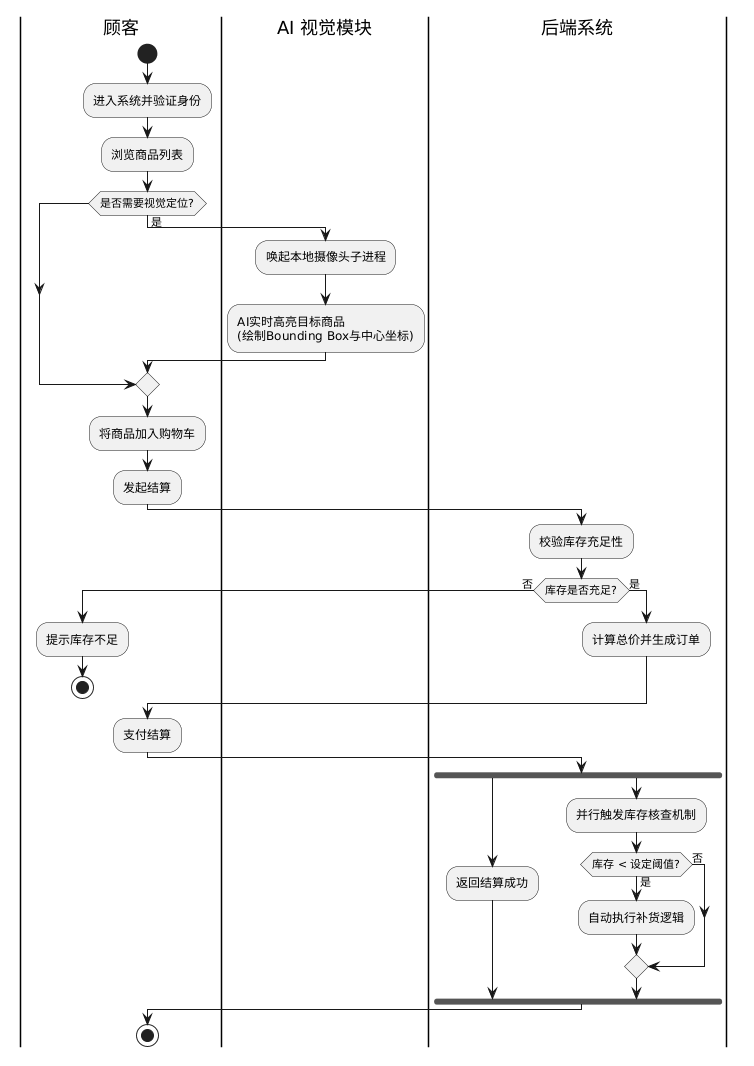
\includegraphics[width=0.88\textwidth]{images/图3-1.png}\\[0.3em]
  {\zihao{-5}图3-1}
\end{center}

\subsubsection{商品上架与基础数据维护业务分析（UC-04）}
本业务流程主要描述商超管理员如何对系统底层的商品字典和库存容量进行初始化及日常维护。

\begin{itemize}[leftmargin=2em]
  \item 业务描述：
\end{itemize}
\begin{enumerate}[leftmargin=2.6em]
  \item 商超管理员登录系统后台管理面板。
  \item 选择“商品录入/更新”功能模块。
  \item 输入商品的英文标识（需严格匹配 YOLO 模型的 names 标签）、零售单价以及入库数量。
  \item 后端系统接收到数据后，对数据库进行 Upsert（更新或插入）防重载校验。
  \item 如果数据库中已存在该商品，则将新入库数量与原有库存进行累加，并以最新填报的价格覆盖旧价格。
  \item 如果是全新商品，则在数据库中插入一条全新记录。
\end{enumerate}

\begin{itemize}[leftmargin=2em]
  \item 角色参与说明：
  \item 商超管理员：数据的提供者，确保录入的商品标识与 AI 视觉模型训练集分类保持强一致性。
  \item 后端系统：数据校验者，保证商品数据的唯一性，防止因重复录入导致数据库出现脏数据。
\end{itemize}

\begin{center}
  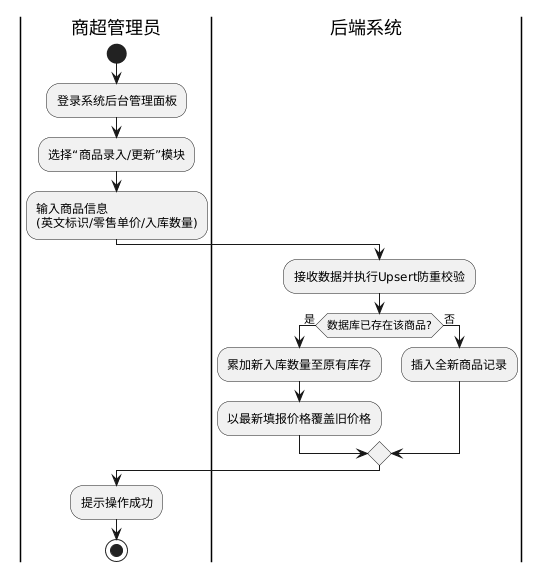
\includegraphics[width=0.88\textwidth]{images/图3-2.png}\\[0.3em]
  {\zihao{-5}图3-2}
\end{center}

\subsection{功能用例分析}

\subsubsection{视觉识别与定位分析（UC-01）}
\begin{itemize}[leftmargin=2em]
  \item 用例名称：视觉识别与物品定位
  \item 用例编号：UC-01
  \item 参与者：顾客
  \item 前置条件：系统后台服务已正常启动；YOLO 模型权重文件已正确加载；操作系统已授予 Python 进程访问本地摄像头的硬件权限。
  \item 主要事件流（Main Flow）：
\end{itemize}
\begin{enumerate}[leftmargin=2.6em]
  \item 顾客浏览系统主界面的货架商品列表，选择目标商品，点击“定位寻物”按钮。
  \item 前端界面锁定该按钮防止重复提交，并通过异步请求（Fetch API）通知后端视觉服务。
  \item 后端视觉处理中心利用 subprocess 模块拉起独立的 YOLO 推理脚本。
  \item 视觉脚本捕捉摄像头实时帧序列，进行图像预处理，喂入 YOLO 模型进行毫秒级目标检测运算。
  \item 模型输出包含分类标签、置信度以及 Bounding Box 坐标（x1, y1, x2, y2）的张量数据。
  \item 系统过滤非目标物品数据，计算目标物品屏幕中心坐标，并在独立的监控窗口上绘制绿色高亮边框与红色中心准星。
  \item 顾客根据屏幕指引在物理货架上准确找到商品。
\end{enumerate}

\begin{itemize}[leftmargin=2em]
  \item 备选事件流（Alternative Flow）：
  \item 物品未找到（A1）：如果在视频流中持续 N 帧未检测到目标类别的置信度 \(\geq\) 预设阈值（如 0.5），则系统在监控窗口上方显示醒目的红色文本提示“未在画面中找到物品”。
  \item 后置条件：顾客完成选购，按 'q' 键释放摄像头资源，系统非阻塞地安全销毁视觉推理子进程。
\end{itemize}

\begin{center}
  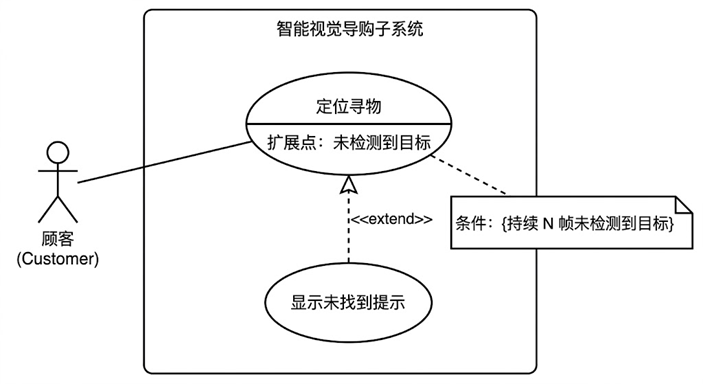
\includegraphics[width=0.88\textwidth]{images/图3-3.png}\\[0.3em]
  {\zihao{-5}图3-3}
\end{center}

\subsubsection{购物车管理与批量结算（UC-03, UC-04）}
\begin{itemize}[leftmargin=2em]
  \item 用例名称：购物车管理与批量结算
  \item 用例编号：UC-03/04（复合用例）
  \item 参与者：顾客
  \item 前置条件：顾客身份已通过登录校验；数据库处于非锁定状态。
  \item 触发条件：顾客完成商品挑选后，主动点击“结算”按钮。
  \item 业务规则：同一商品重复加入购物车时仅累加数量；结算金额统一保留两位小数；结算接口需校验一次性请求标识（Token）以避免重复扣款。
  \item 主要事件流（Main Flow）：
\end{itemize}
\begin{enumerate}[leftmargin=2.6em]
  \item 顾客在系统前端货架列表中点击商品旁的“+ 加入购物车”按钮。
  \item 前端动态更新内存中的购物车对象，实时计算并显示当前金额总计。
  \item 顾客可在购物车面板中增减商品数量、删除单项商品，并实时查看金额变化。
  \item 顾客点击“一键刷脸结算”按钮。
  \item 前端将完整的 JSON 清单请求发送至后端结算 API。
  \item 后端开启数据库事务。遍历清单，锁定 products 表对应行记录，执行原子扣减操作：stock = stock - buy\_quantity。
  \item 计算所有单品的花费金额总计。在 orders 表中为该顾客写入一条全新的销售订单记录。
  \item 后端返回订单摘要（订单 ID、金额、时间戳、购买清单），前端进行成功态渲染。
  \item 提交数据库事务。前端清空本地购物车缓存，向顾客展示模拟扣款成功的回执界面（包含订单 ID、消费金额）。
\end{enumerate}

\begin{itemize}[leftmargin=2em]
  \item 异常事件流（Exception Flow）：
  \item 库存不足（E1）：在遍历结算清单时，系统检测到某单品的现有库存量小于其购买量。后端拦截交易，回滚数据库事务，并向前端返回报错信息：“【商品 A】库存不足，结算失败！”。
  \item 重复提交（E2）：当顾客连续点击结算按钮导致同一 Token 重复到达时，后端仅受理首个请求，其余请求返回“订单已处理”提示，不再进行二次扣减。
  \item 订单写入失败（E3）：若订单写入阶段发生数据库异常，系统执行事务回滚，并提示“系统繁忙，请稍后重试”。
  \item 后置条件：订单状态被持久化存储；前端恢复初始货架状态；系统静默触发库存预警用例（UC-07）。
\end{itemize}

\begin{center}
  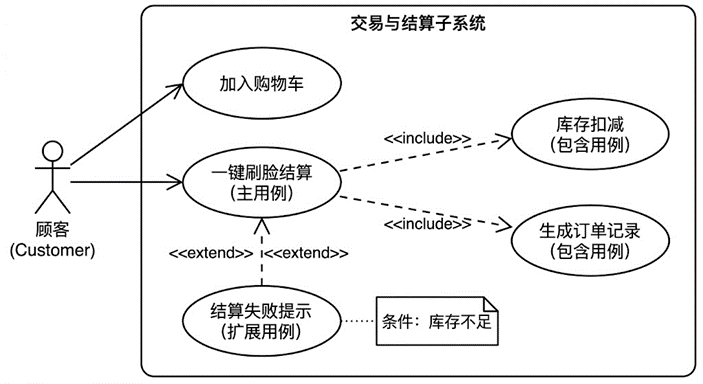
\includegraphics[width=0.88\textwidth]{images/图3-4.png}\\[0.3em]
  {\zihao{-5}图3-4}
\end{center}

\subsubsection{商品信息维护管理（UC-05）}
\begin{itemize}[leftmargin=2em]
  \item 用例名称：商品信息维护管理
  \item 用例编号：UC-05
  \item 参与者：商超管理员
  \item 前置条件：管理员已通过鉴权登录系统后台。
  \item 触发条件：管理员进入“商品维护”页面并提交新增或更新请求。
  \item 业务规则：商品英文标识必须与模型类别名一致；单价必须大于 0；库存数量必须为非负整数。
  \item 主要事件流（Main Flow）：
\end{itemize}
\begin{enumerate}[leftmargin=2.6em]
  \item 管理员进入后台维护面板，输入商品的英文标识名称（需匹配 YOLO 推理脚本分类标签）。
  \item 管理员选择“新品上架”或“库存补录”模式，输入单价和入库数量（例如 50）。
  \item 管理员点击提交。后端拦截该数据。
  \item 后端执行字段合法性校验（名称、价格、库存）。
  \item 系统执行 Upsert 逻辑：先在数据库中检索是否存在同名商品。
  \item 如果存在，则更新价格并将新入库量累加至旧库存（stock = existing\_stock + 50）。
  \item 如果不存在，则创建全新商品记录（INSERT），设置初始库存。
  \item 系统记录本次操作日志（操作者、时间、变更前后值），用于审计追踪。
\end{enumerate}

\begin{itemize}[leftmargin=2em]
  \item 异常事件流（Exception Flow）：
  \item 标签不匹配（E1）：商品名称与模型类别集不一致时，系统拒绝写入并提示“商品标签未在视觉模型中注册”。
  \item 字段非法（E2）：当价格小于等于 0 或库存为负值时，系统返回参数校验失败信息。
  \item 数据库不可用（E3）：写入过程中数据库连接异常，系统返回失败信息并保留原数据。
  \item 后置条件：管理员接收前端“数据维护成功”的提示信息；本地数据库数据已同步更新。
\end{itemize}

\begin{center}
  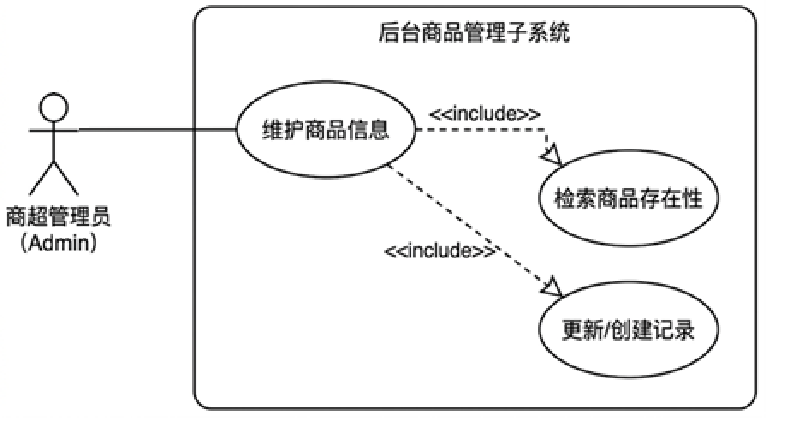
\includegraphics[width=0.88\textwidth]{images/图3-5.png}\\[0.3em]
  {\zihao{-5}图3-5}
\end{center}

\subsubsection{销售数据统计大盘（UC-06）}
\begin{itemize}[leftmargin=2em]
  \item 用例名称：销售数据统计大盘
  \item 用例编号：UC-06
  \item 参与者：商超管理员
  \item 前置条件：系统处于运营状态，数据库中存在历史订单记录。
  \item 触发条件：管理员打开“统计报表”页面或主动点击“刷新报表”。
  \item 业务规则：统计周期默认按自然日聚合；金额统一以人民币元为单位保留两位小数；Top 榜单按销量降序展示。
  \item 主要事件流（Main Flow）：
\end{itemize}
\begin{enumerate}[leftmargin=2.6em]
  \item 管理员进入后台数据报表面板。
  \item 前端自动向后端 API 请求聚合统计数据。
  \item 后端利用 SQL 聚合函数在 orders 表上执行 Group By 操作。计算核心指标：当天总营业额、总单量、总销售件数。计算销售件数 Top 5 畅销商品排行榜。
  \item 系统将计算结果封装为标准 JSON 格式并返回。
  \item 前端利用图表库（如简单的 html/js 表格）将数据进行可视化渲染呈现给管理员。
  \item 管理员可选择导出当天统计快照（CSV）用于离线分析。
\end{enumerate}

\begin{itemize}[leftmargin=2em]
  \item 异常事件流（Exception Flow）：
  \item 无订单数据（E1）：若当前统计周期内无有效订单，系统返回零值统计并提示“暂无销售数据”。
  \item 查询超时（E2）：聚合查询超时则返回缓存数据，并提示“当前展示为最近一次统计快照”。
  \item 可视化渲染失败（E3）：前端图表渲染异常时自动降级为表格文本展示。
  \item 后置条件：统计结果被写入缓存层，供后续页面快速读取。
\end{itemize}

\begin{center}
  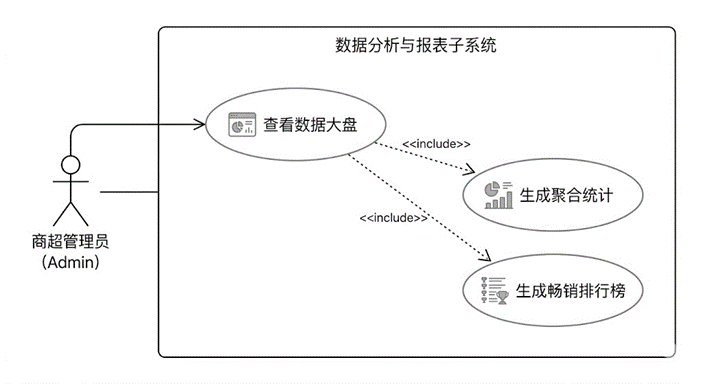
\includegraphics[width=0.88\textwidth]{images/图3-6.png}\\[0.3em]
  {\zihao{-5}图3-6}
\end{center}

\subsubsection{阈值预警与自动补货（UC-07）}
\begin{itemize}[leftmargin=2em]
  \item 用例名称：阈值预警与自动补货
  \item 用例编号：UC-07
  \item 参与者：系统后台（守护进程）、模拟供应商
  \item 前置条件：结算事务（UC-04）成功执行且提交数据库。
  \item 触发条件：订单完成后库存发生变化，触发库存巡检任务。
  \item 业务规则：预警阈值支持按商品维度独立配置；同一商品在同一巡检周期内仅触发一次补货请求；补货默认批量为 50 件。
  \item 主要事件流（Main Flow）：
\end{itemize}
\begin{enumerate}[leftmargin=2.6em]
  \item 系统结算逻辑完成后，触发库存核查钩子（Hook）。
  \item 系统查询刚才被扣减库存的商品（例如 A）在 products 表中最新的剩余库存量。
  \item 系统判断：剩余库存 \(\leq\) 预警阈值（默认=3）？
  \item 如果是，系统后台自动组装标准化补货工单（JSON），包含：请求的外部供应商 API 地址、商品英文名、补货量（例如固定 +50 件）。
  \item 系统将报文 POST 发送至外部模拟供应商的 API 接口。
  \item 接收到供应商返回的发货确认 JSON 回执后，系统在本地数据库强制追加该商品库存（stock = stock + 50），并生成补货系统日志供管理员查阅。
  \item 系统向管理员消息中心推送“自动补货已执行”的通知，附带商品名称与补货数量。
\end{enumerate}

\begin{itemize}[leftmargin=2em]
  \item 异常事件流（Exception Flow）：
  \item 供应商接口不可达（E1）：若外部 API 请求失败，系统将补货任务写入重试队列并按指数退避策略重试。
  \item 供应商回执异常（E2）：当回执字段缺失或状态码非法时，系统不更新库存并标记任务为“人工复核”。
  \item 并发冲突（E3）：当库存记录被其他事务占用时，系统等待短时重试，超过阈值后转入补偿任务队列。
  \item 后置条件：供应链补给流程完成，无需人工干预。
\end{itemize}

\begin{center}
  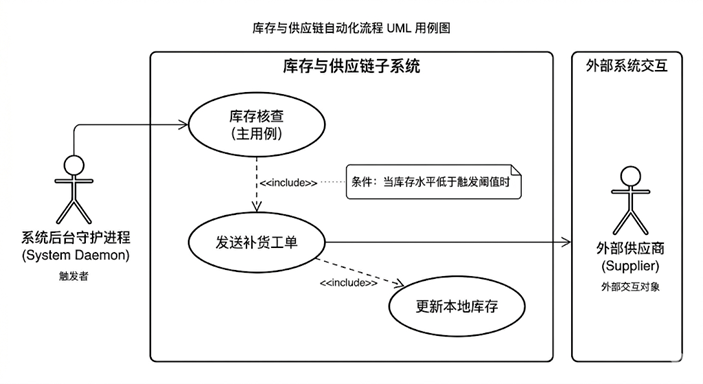
\includegraphics[width=0.88\textwidth]{images/图3-7.png}\\[0.3em]
  {\zihao{-5}图3-7}
\end{center}

\subsection{数据流分析}
本节通过数据流图（DFD）自顶向下地分析系统内外部的数据流转过程，主要包含顶层数据流图和一层数据流图。

\subsubsection{顶层数据流图}
顶层数据流图主要界定了“智能零售系统”的边界，以及它与外部实体（顾客、管理员、供应商）之间的顶层数据交互。

\begin{center}
  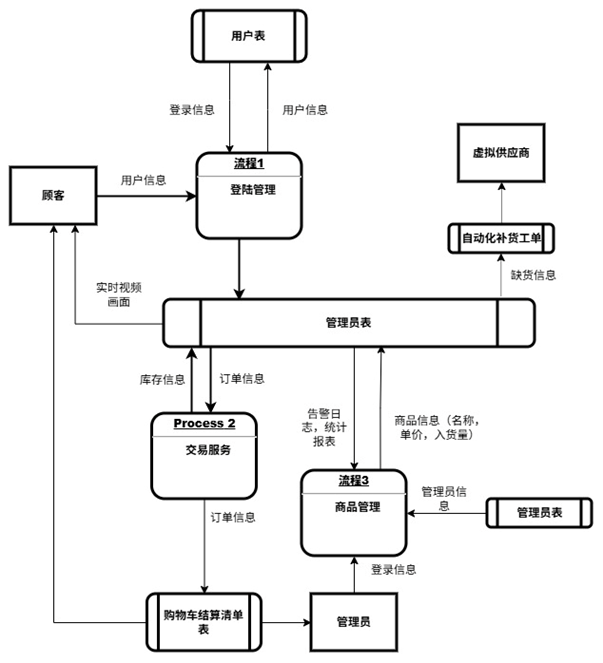
\includegraphics[width=0.88\textwidth]{images/图3-8.png}\\[0.3em]
  {\zihao{-5}图3-8}
\end{center}

\subsubsection{一层数据流图}
一层数据流图主要界定了“智能零售系统”的边界，以及它与外部实体（顾客、管理员、供应商）之间的顶层数据交互。

  \quad
  \quad
\begin{center}
  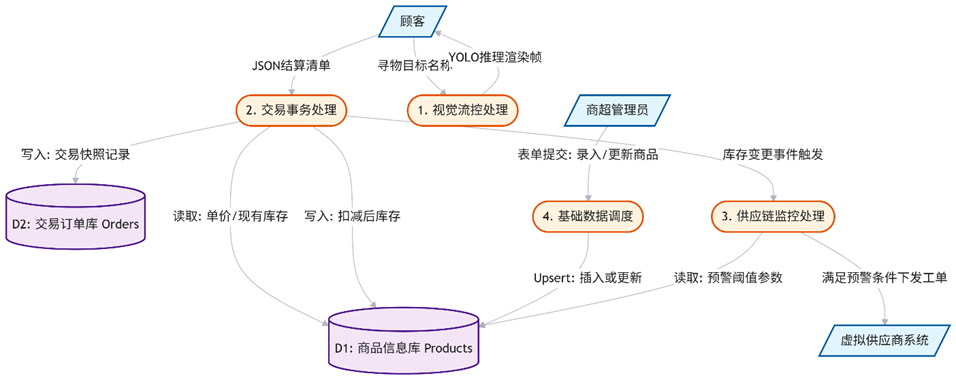
\includegraphics[width=0.88\textwidth]{images/图3-9.png}\\[0.3em]
  {\zihao{-5}图3-9}
\end{center}

\section{非功能性需求}

\subsection{性能需求}
\begin{itemize}[leftmargin=2em]
  \item 算法推理延迟：在配备 NVIDIA GPU 的计算环境下，YOLOv8 模型对单帧图像的推理时间应 \(\leq\) 30ms，保证视频流视觉无明显卡顿（\(>\)25 FPS）。
  \item 接口响应时间：除视觉处理外的所有在线数据 API（如获取商品列表、批量结算），在本地回环网络下的响应时间必须 \(\leq\) 200ms。
  \item 识别准确率：在光照充足、商品无严重遮挡的理想商超环境下，算法对已训练目标的识别召回率（Recall）应达到 90\% 以上。
\end{itemize}

\subsection{安全性需求}
\begin{itemize}[leftmargin=2em]
  \item 并发隔离：视觉推理模块必须与后端 Web 服务器（Uvicorn）在不同进程中运行（通过子进程拉起），防止因摄像头异常或显存溢出导致整个收银系统崩溃。
  \item 数据一致性：结算扣款与库存扣减必须置于同一个数据库事务（Transaction）中处理。若库存不足，必须全部回滚，严禁出现“钱已扣但库存未减”的脏写现象。
  \item 防注入攻击：前后端数据交互严格遵守 RESTful 规范，利用 Pydantic 模型进行强制数据类型校验，防止恶意的 SQL 注入或格式越界。
\end{itemize}

\subsection{易用性需求}
\begin{itemize}[leftmargin=2em]
  \item 极简部署：系统需提供 requirements.txt 或 environment.yml，确保在一台全新计算机上可通过简单的命令实现一键环境复原。
  \item UI 容错机制：前端界面对所有网络请求异常（如后端服务未启动、接口 404）进行捕获，并以弹窗或红色醒目文字的形式给出人类可读的提示（如“网络错误，无法连接后端”），禁止出现控制台级报错直接暴露给普通用户。
\end{itemize}

\swjtuChapter{系统概要设计报告}

% 去掉章节前缀，使用 1 / 1.1 / 1.1.1 的编号体系
\setcounter{section}{0}
\renewcommand{\thesection}{\arabic{section}}
\renewcommand{\thesubsection}{\thesection.\arabic{subsection}}
\renewcommand{\thesubsubsection}{\thesubsection.\arabic{subsubsection}}

%%% ==================== 1 引言 ==================== %%%
\section{引言}

\subsection{编写目的}
本文档为“零售物品智能识别系统”的概要设计报告，旨在将《软件需求规格说明书》中确定的功能性与非功能性需求转化为可实施的系统体系结构、模块划分、接口契约与数据库方案。文档将作为后续详细设计、编码实现和系统测试的核心依据，确保各子系统在架构层面达成一致。

\subsection{项目背景}
本系统面向中小型零售商超场景，利用 YOLOv8 目标检测算法与计算机视觉技术，结合 Web 全栈开发能力，构建一套集“视觉导购、自助结算、智能库存管理”于一体的闭环平台。系统由四个子系统组成：Java 后端服务（retail-server）、Vue3 管理端（retail-admin-pro）、微信小程序客户端（retail-customer）以及 Python AI 服务（retail-ai），共同支撑商品管理、购物车结算、库存预警、摄像头巡检和智能搜索等核心业务。

\subsection{相关术语}
\begin{itemize}[leftmargin=2em]
  \item Spring Boot：基于 Java 的企业级应用开发框架，本系统采用 3.3 版本，运行于 Java 21 平台。
  \item MyBatis-Plus：MyBatis 的增强工具，简化数据持久层的 CRUD 操作。
  \item JWT（JSON Web Token）：一种无状态的用户鉴权令牌机制，本系统用于管理端和小程序端的登录凭证。
  \item Vue3 + Vite：前端渐进式框架与构建工具，管理端基于 TypeScript 和 Element Plus 组件库。
  \item 微信小程序：运行于微信客户端的轻应用，本系统的 C 端入口。
  \item FastAPI：Python 高性能异步 Web 框架，本系统 AI 服务的运行载体。
  \item OpenCV：开源计算机视觉库，用于摄像头采集与图像编解码。
  \item YOLOv8：新一代实时目标检测算法，用于货架商品识别。
  \item Redis：内存键值数据库，本系统用于购物车存储、Token 鉴权缓存与推荐流缓存。
  \item RESTful API：基于 HTTP 方法的资源型接口风格，系统内外部通信均采用此规范。
  \item DTO / VO：数据传输对象 / 视图对象，分别用于接收请求参数和封装响应数据。
  \item MJPEG：Motion JPEG 视频流协议，用于摄像头实时画面传输。
  \item BFF（Backend For Frontend）：为前端量身定制的后端服务层模式。
\end{itemize}

\subsection{参考文献}
\begin{enumerate}[leftmargin=2em]
  \item 《软件工程：实践者的研究方法》（第9版），Roger S. Pressman.
  \item Spring Boot 3.3 官方文档 \textnormal{https://spring.io/projects/spring-boot}
  \item Vue3 官方文档 \textnormal{https://vuejs.org/}
  \item 微信小程序开发指南 \textnormal{https://developers.weixin.qq.com/miniprogram/dev/}
  \item FastAPI 官方文档 \textnormal{https://fastapi.tiangolo.com/}
  \item YOLOv8（Ultralytics）官方文档 \textnormal{https://docs.ultralytics.com/}
  \item MyBatis-Plus 官方文档 \textnormal{https://baomidou.com/}
\end{enumerate}

%%% ==================== 2 系统体系结构设计 ==================== %%%
\section{系统体系结构设计}

\subsection{系统特点分析}
\begin{enumerate}[leftmargin=2em]
  \item \textbf{四端分离架构}：系统由 Java 后端（retail-server）、Vue3 管理前端（retail-admin-pro）、微信小程序（retail-customer）和 Python AI 服务（retail-ai）四个独立子系统组成，各自拥有独立的代码仓库、构建工具和运行环境，通过 RESTful HTTP/JSON 协议进行通信。
  \item \textbf{统一 API 网关}：retail-server 同时承担 BFF 角色，为管理端提供 \texttt{/api/*} 接口，为小程序提供 \texttt{/api/applet/*} 接口，并通过 JWT 拦截器统一鉴权。
  \item \textbf{AI 能力独立部署}：retail-ai 作为独立微服务运行在 8000 端口，仅暴露视觉识别与文本检索能力，retail-server 通过 RestTemplate 进行 HTTP 中转调用，二者可独立扩缩容。
  \item \textbf{Redis 热数据缓存}：购物车数据与推荐流等高频读写数据通过 Redis 缓存，购物车使用 Hash 结构（\texttt{cart:user:\{userId\}}）持久化，推荐流设置 TTL 自动过期，降低数据库查询压力。
  \item \textbf{定时巡检机制}：后端内置基于 ThreadPoolTaskScheduler 的摄像头定时巡检调度器，可动态调整间隔和批次大小，支持手动触发全量扫描。
\end{enumerate}

\subsection{系统体系结构设计}

\subsubsection{系统体系结构模式}
本系统整体采用\textbf{分层架构 + 微服务}的混合体系结构模式：
\begin{itemize}[leftmargin=2em]
  \item \textbf{分层架构}：retail-server 内部严格遵循 Controller → Service → Mapper 三层分层，Controller 负责请求路由与参数校验，Service 封装业务逻辑，Mapper 通过 MyBatis-Plus 完成数据持久化。
  \item \textbf{微服务拆分}：AI 视觉能力被独立为 retail-ai 微服务，与主后端通过 HTTP 协议松耦合集成，故障隔离性好。
  \item \textbf{前端 MVC/MVVM}：管理端采用 Vue3 的组合式 API + Pinia 状态管理，小程序采用微信原生框架的页面/组件模型。
  \item \textbf{BFF 模式}：retail-server 根据不同前端（管理端 / 小程序）的需求，提供差异化的接口路径和返回结构。
\end{itemize}

\subsubsection{系统体系结构设计}

\paragraph{（1）逻辑视图设计}

\begin{center}
  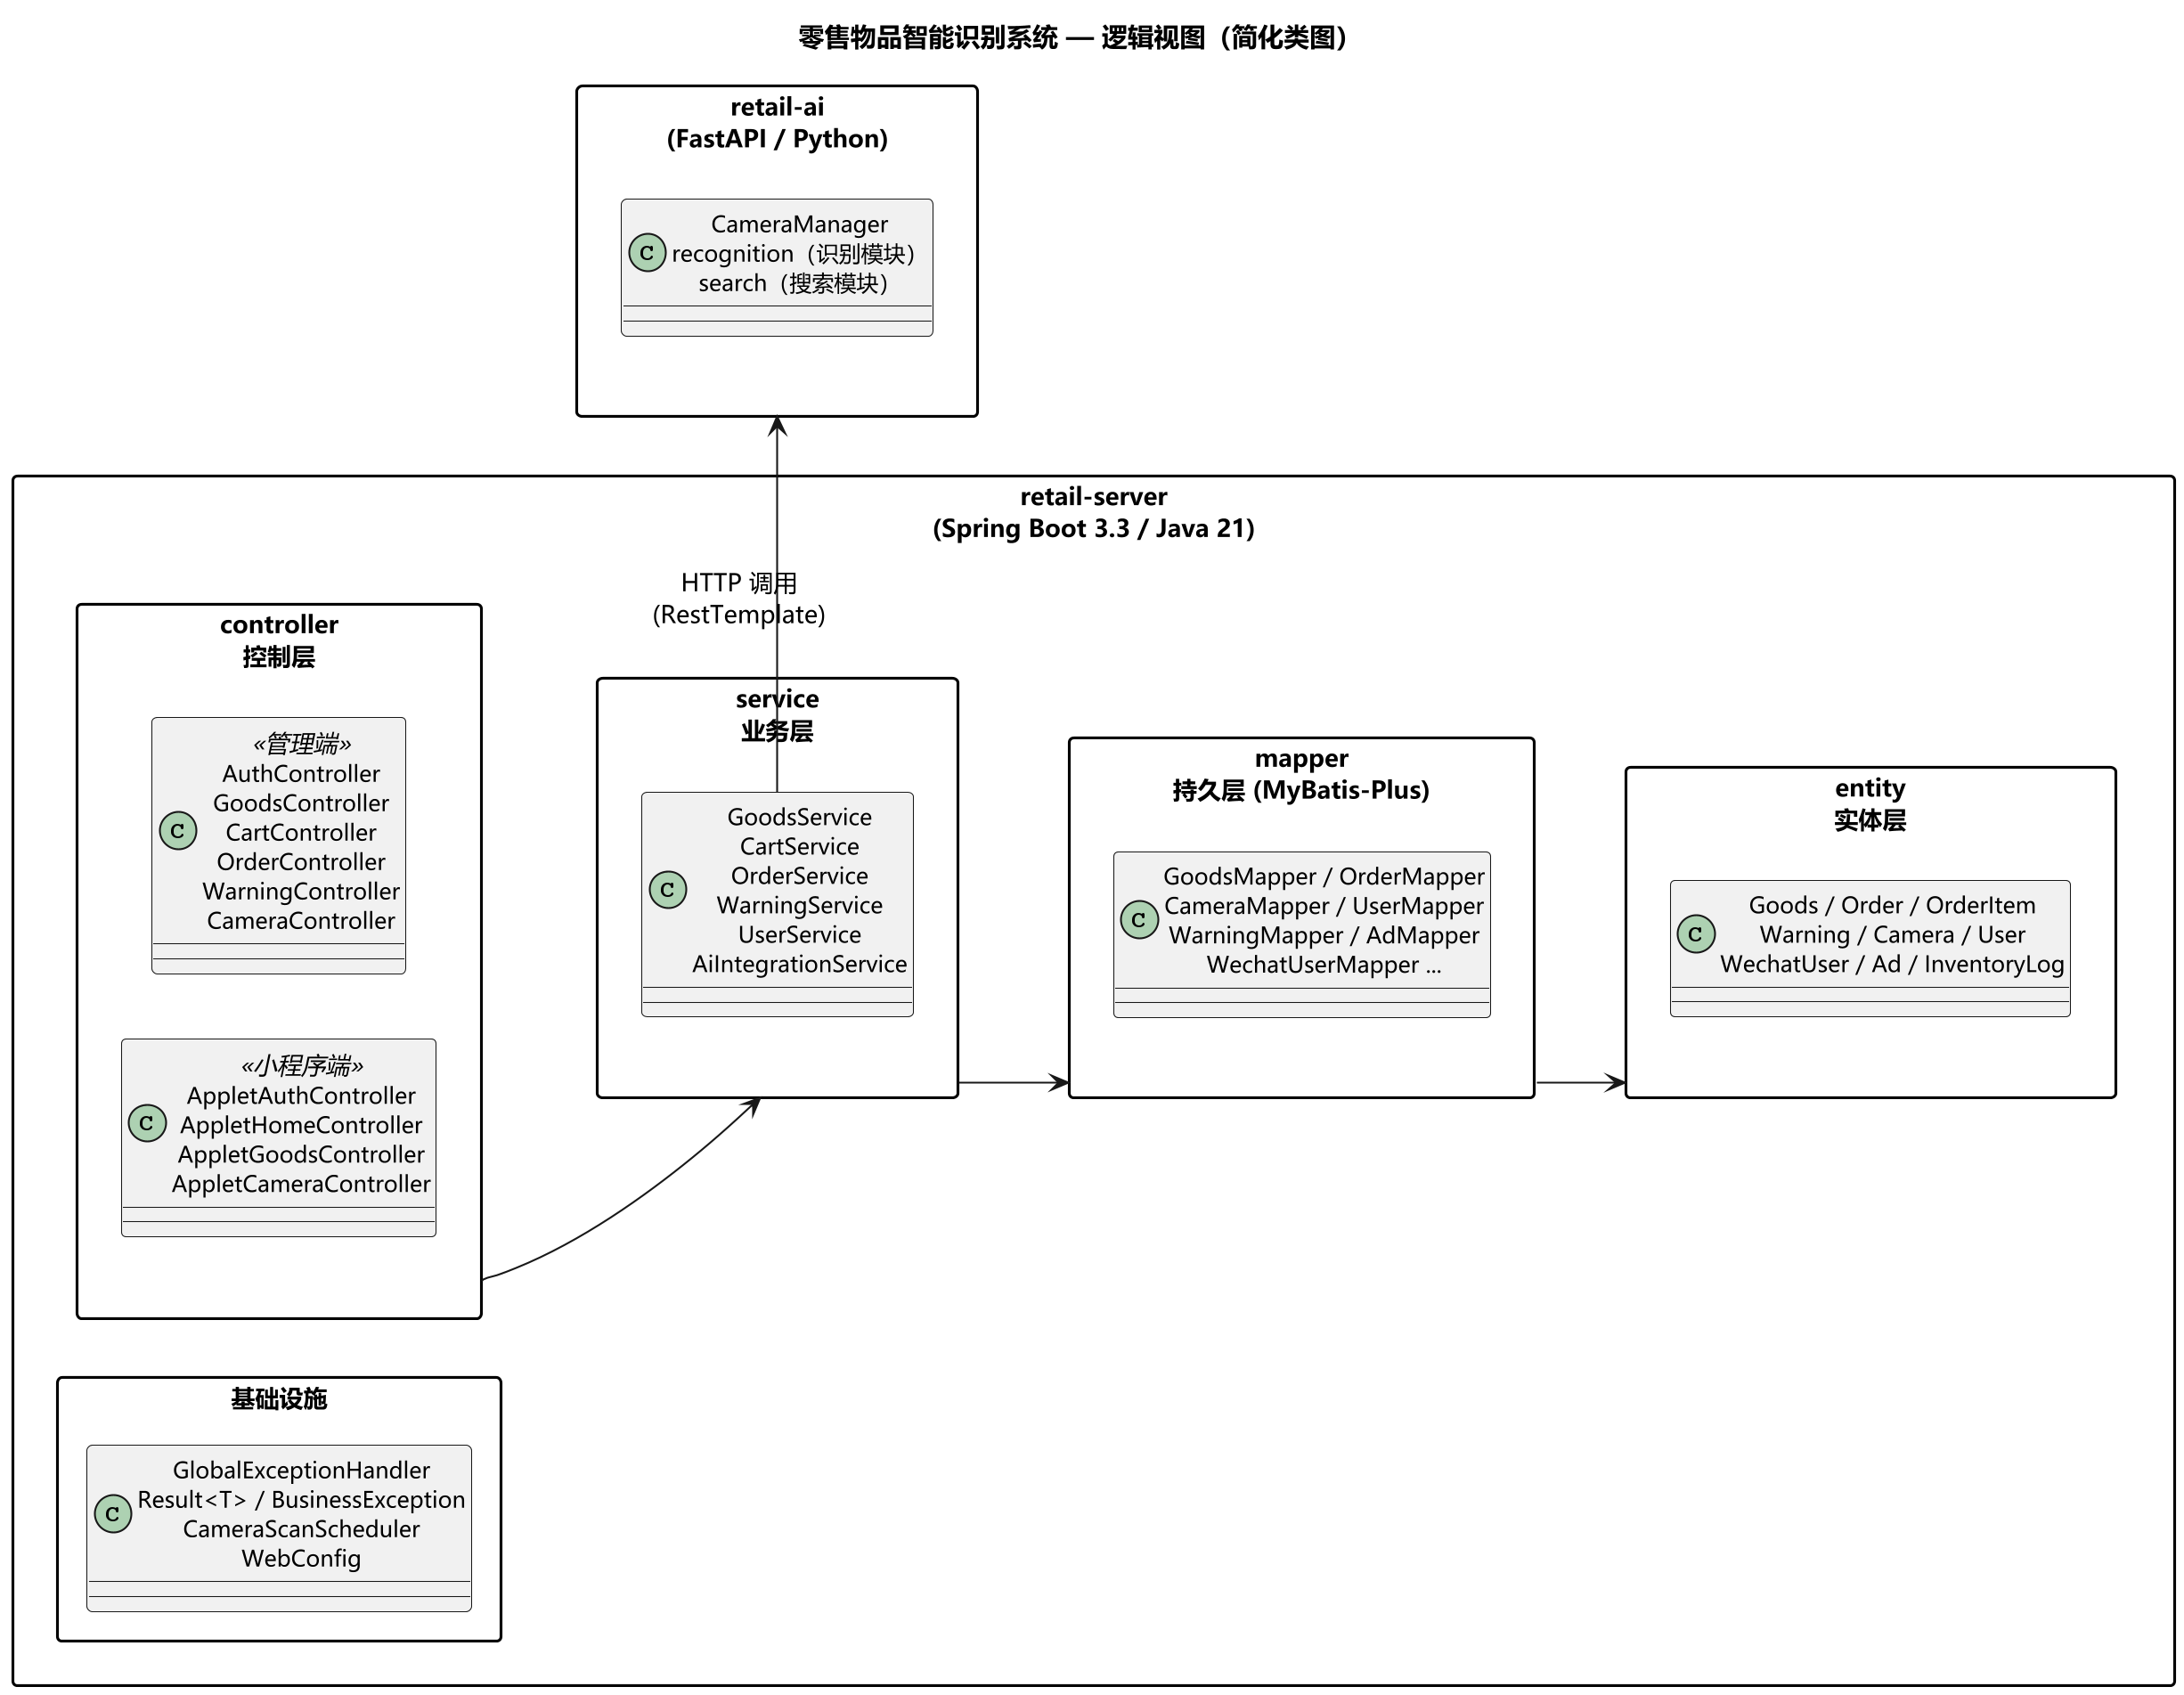
\includegraphics[width=0.95\textwidth]{images/fig-logic-view.png}\\[0.3em]
  {\zihao{-5}图2-1\quad 系统逻辑视图——简化类图}
\end{center}

retail-server 后端代码按照职责划分为以下核心包：

\begin{itemize}[leftmargin=2em]
  \item \textbf{controller 包}：面向管理端的控制器包括 AuthController（登录鉴权）、GoodsController（商品 CRUD）、CartController（购物车）、OrderController（订单结算）、WarningController（库存告警）、CameraController（摄像头管理与巡检调度）、AdminWarningController（管理端告警列表）、FileController（文件上传）；面向小程序的控制器以 \texttt{applet} 子包组织，包括 AppletAuthController、AppletHomeController、AppletGoodsController、AppletOrderController，以及 AppletCameraController（扫码识别）。
  \item \textbf{service 包}：业务逻辑层包括 GoodsService、CartService、OrderService、WarningService、UserService、OrderDetailService、AiIntegrationService（封装对 Python AI 服务的调用）及 AsyncCartService（异步购物车操作）。每个接口均有对应的 Impl 实现类。
  \item \textbf{mapper 包}：数据持久层包含 GoodsMapper、OrderMapper、OrderItemMapper、OrderDetailMapper、CameraMapper、UserMapper、WechatUserMapper、WarningMapper、InventoryLogMapper、AdMapper、GoodsCategoryMapper 共 11 个 MyBatis-Plus Mapper 接口，均继承 BaseMapper 泛型类。
  \item \textbf{entity 包}：数据实体类与数据库表一一映射，包括 Goods、Order、OrderItem、Warning、Camera、User、WechatUser、Ad、GoodsCategory、InventoryLog 等。
  \item \textbf{dto / vo 包}：DTO 用于接收前端请求（LoginRequest、CartDTO、AppletScanRequest、CameraBindRequest 等），VO 用于封装响应数据（AppletGoodsVO、CartVO、OrderVO、AppletAdVO 等）。
  \item \textbf{config 包}：全局配置类包括 WebConfig（JWT 拦截器注册与静态资源映射）、MybatisPlusConfig（分页插件）、RestTemplateConfig（HTTP 客户端）、TaskSchedulerConfig（线程池调度器）、CorsConfig（跨域配置）。
  \item \textbf{exception 包}：统一异常处理，BusinessException 为自定义业务异常，GlobalExceptionHandler 通过 \texttt{@RestControllerAdvice} 捕获所有异常并返回统一 JSON 结构。
  \item \textbf{scheduler 包}：CameraScanScheduler 实现摄像头定时巡检，支持动态配置间隔和批次大小、手动触发、生命周期管理。
  \item \textbf{common 包}：Result 类封装统一的接口返回结构（code + message + data）。
  \item \textbf{context 包}：UserContext 基于 ThreadLocal 存储当前登录用户 ID，由 JwtAuthInterceptor 在请求进入时写入。
\end{itemize}

retail-ai 服务按功能划分为三个模块：
\begin{itemize}[leftmargin=2em]
  \item \textbf{camera 模块}：CameraManager 类实现线程安全的摄像头管理（引用计数 + 空闲超时回收），camera routes 提供探测可用摄像头、单帧获取、MJPEG 视频流、资源释放等端点。
  \item \textbf{recognition 模块}：detector 模块封装 YOLO 目标检测逻辑（演示环境为模拟检测器），recognition routes 提供中心点识别和批量货架识别两个端点。
  \item \textbf{search 模块}：search routes 提供基于 Jaccard 相似度的文本关键词检索端点。
\end{itemize}

\vspace{1em}
\paragraph{（2）开发及运行视图设计}

\begin{center}
  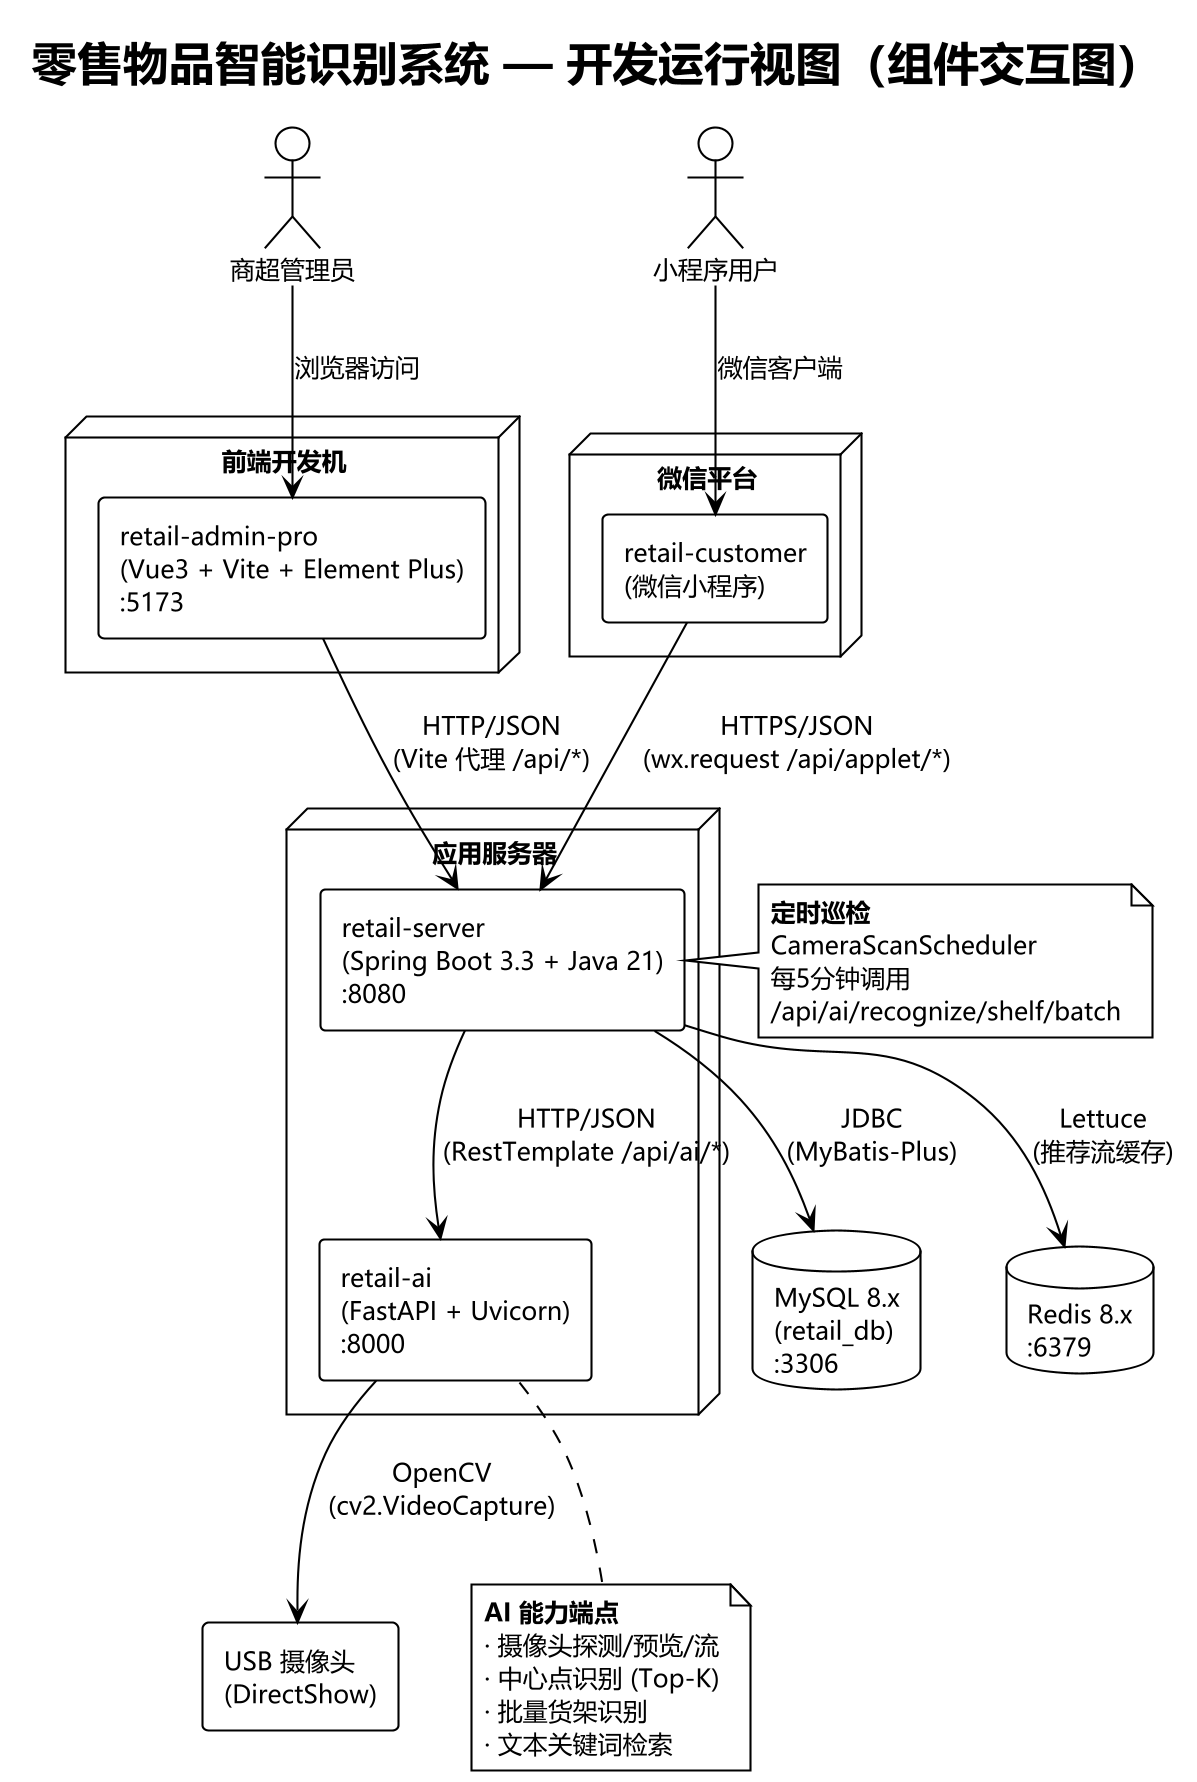
\includegraphics[width=0.95\textwidth]{images/fig-component-view.png}\\[0.3em]
  {\zihao{-5}图2-2\quad 系统开发运行视图——组件交互图}
\end{center}

系统开发与运行视图从子系统交互维度展示了四端之间的协作关系：

\begin{itemize}[leftmargin=2em]
  \item \textbf{retail-admin-pro}（Vue3 + Vite，开发端口 5173）：通过 Vite 反向代理将 \texttt{/api} 请求转发至 retail-server:8080。构建工具为 pnpm + Vite，使用 TypeScript 编写，集成 Element Plus 组件库、Axios HTTP 客户端、Pinia 状态管理和 Vue Router 路由。
  \item \textbf{retail-customer}（微信小程序）：运行于微信客户端，通过 \texttt{wx.request} 调用 retail-server 的 \texttt{/api/applet/*} 接口。使用微信原生框架，页面包括首页（index）、搜索（search）、购物车（cart）、扫码（scan）、用户中心（user）、订单（order）、商品详情（goods）、充值（recharge）、支付（payment）等。
  \item \textbf{retail-server}（Spring Boot 3.3 + Java 21，端口 8080）：通过 Maven 构建，依赖 spring-boot-starter-web、mybatis-plus-spring-boot3-starter、spring-boot-starter-data-redis、jjwt 等。启动后监听 8080 端口，接受管理端和小程序的 REST 请求。需要 AI 能力时，通过 RestTemplate 以同步 HTTP 调用 retail-ai。内置 CameraScanScheduler 定时（默认每 5 分钟）批量调用 retail-ai 的货架识别端点进行巡检。
  \item \textbf{retail-ai}（FastAPI + Uvicorn，端口 8000）：通过 pip 安装依赖（fastapi、uvicorn、opencv-python、numpy、pydantic），启动后监听 8000 端口，仅接受来自 retail-server 的内部调用。使用 OpenCV 进行摄像头操作，通过线程安全的 CameraManager 管理摄像头生命周期。
\end{itemize}

运行时数据流如下：
\begin{enumerate}[leftmargin=2em]
  \item 用户在管理端或小程序发起请求 → 到达 retail-server 的 Controller 层。
  \item Controller 调用 Service 层执行业务逻辑，Service 层通过 Mapper 层访问 MySQL 数据库。
  \item 若业务涉及 AI 能力（文本搜索、图像识别、摄像头预览），Service 或 Controller 通过 RestTemplate 向 retail-ai 发起 HTTP 请求。
  \item retail-ai 执行视觉推理或文本检索后返回 JSON 结果。
  \item retail-server 整合数据库数据与 AI 结果，封装为统一 Result 结构返回前端。
  \item 推荐流等热点数据写入 Redis 缓存，后续请求直接从缓存读取。
\end{enumerate}

\paragraph{（3）部署视图设计}

\begin{center}
  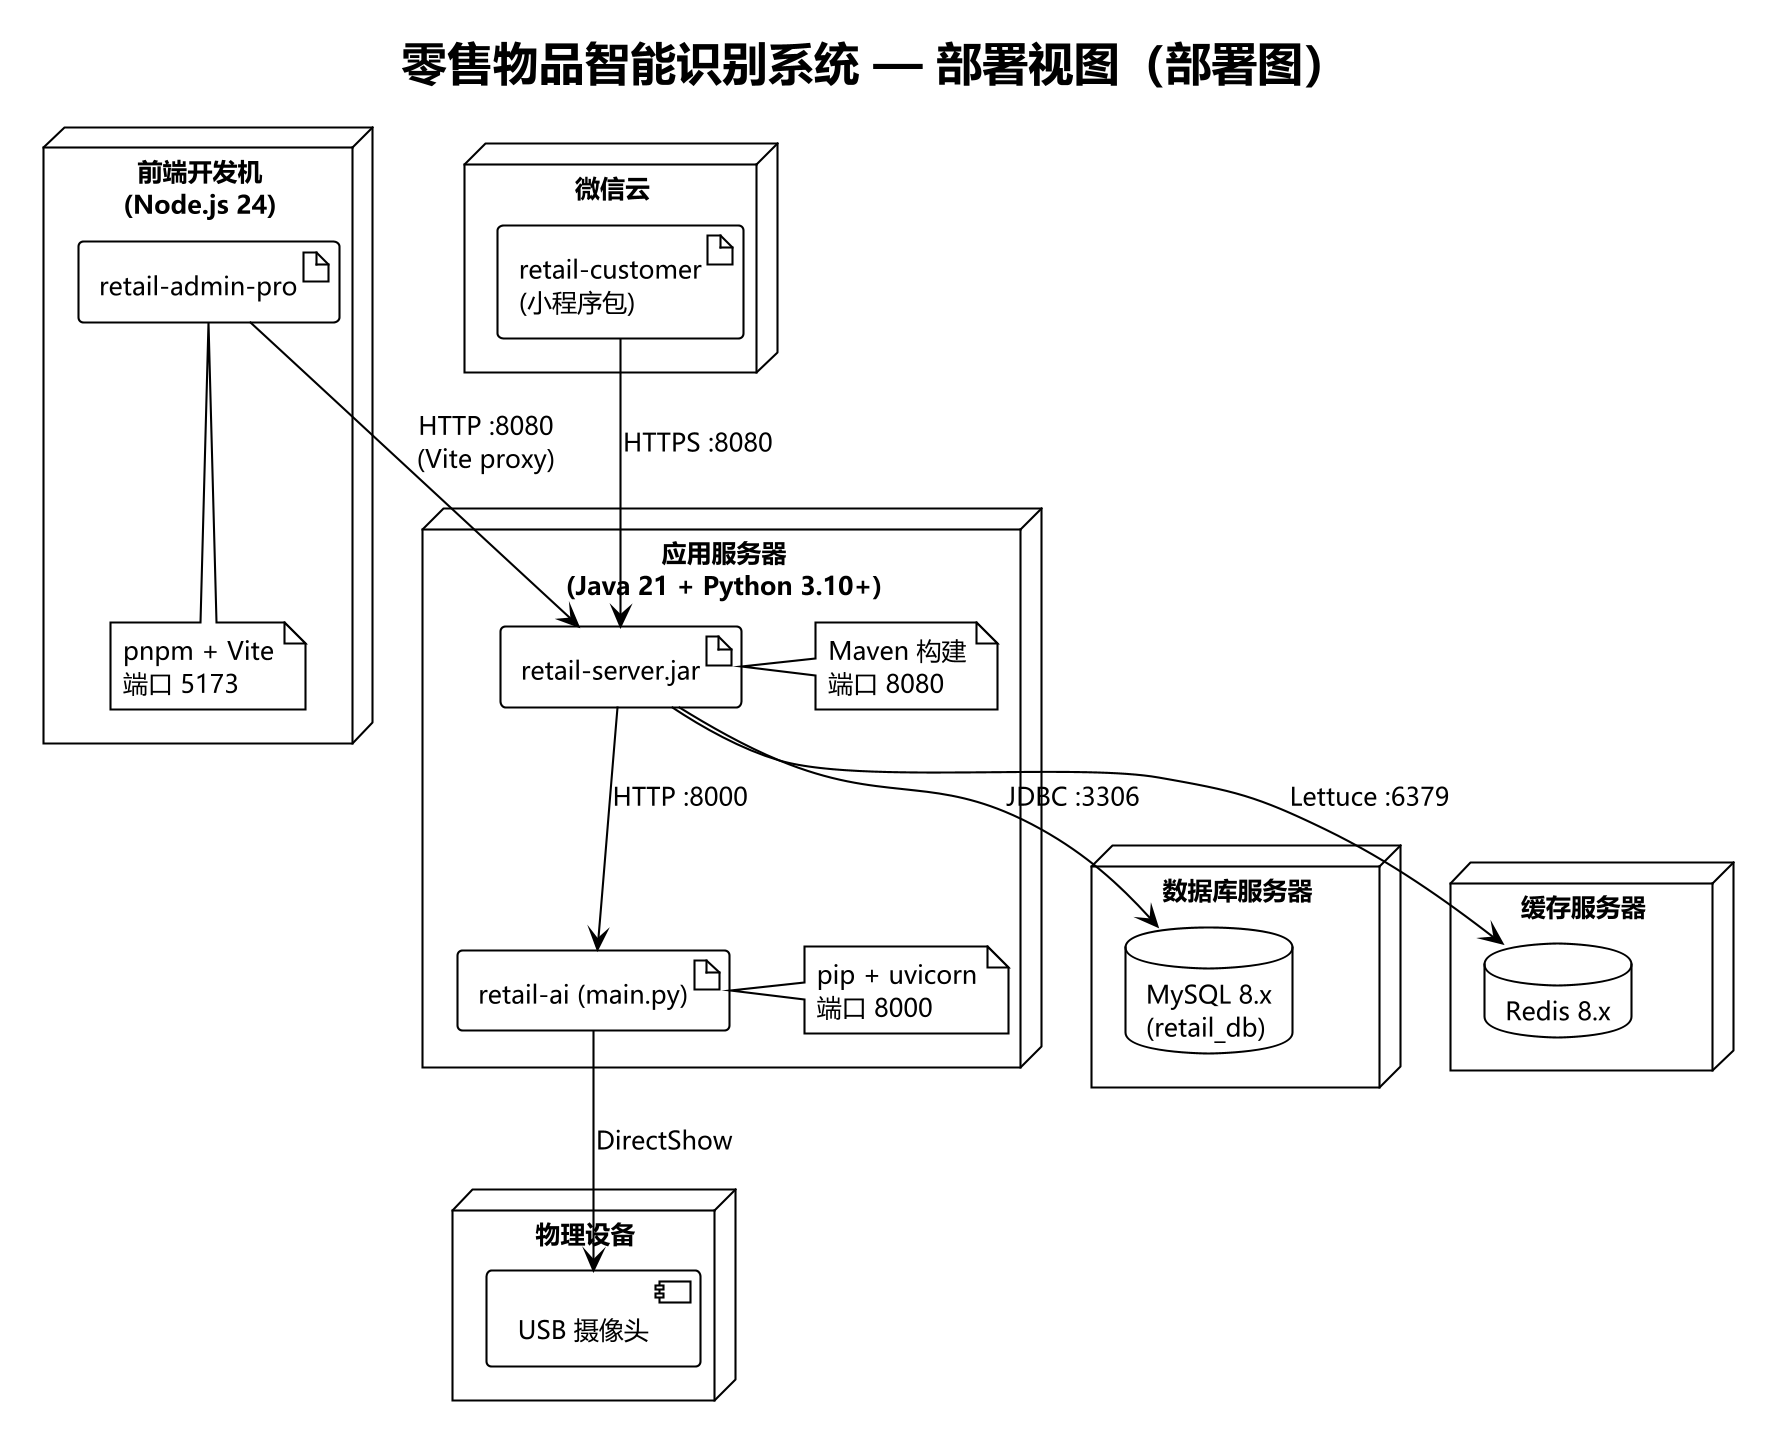
\includegraphics[width=0.88\textwidth]{images/fig-deploy-view.png}\\[0.3em]
  {\zihao{-5}图2-3\quad 系统部署视图——部署图}
\end{center}

系统各组件部署节点说明如下：

\begin{center}
  \renewcommand{\arraystretch}{1.4}
  \zihao{5}
  \begin{tabular}{|>{\centering\arraybackslash}m{2.5cm}|>{\centering\arraybackslash}m{6cm}|>{\centering\arraybackslash}m{1.5cm}|>{\centering\arraybackslash}m{2.8cm}|}
    \hline
    \textbf{部署节点} & \textbf{运行内容}                     & \textbf{端口} & \textbf{运行环境}   \\ \hline
    应用服务器         & retail-server（Spring Boot）        & 8080        & Java 21 + Maven \\ \hline
    应用服务器         & retail-ai（FastAPI + Uvicorn）      & 8000        & Python 3.10+    \\ \hline
    前端开发机         & retail-admin-pro（Vite Dev Server） & 5173        & Node.js 24      \\ \hline
    微信平台          & retail-customer（小程序包）             & —           & 微信客户端           \\ \hline
    数据库服务器        & MySQL 8.x（retail\_db 数据库）         & 3306        & —               \\ \hline
    缓存服务器         & Redis 8.x                         & 6379        & —               \\ \hline
    物理设备          & USB 摄像头                           & —           & DirectShow      \\ \hline
  \end{tabular}
  \\[0.3em]
  {\zihao{-5}表2-1\quad 系统部署节点说明}
\end{center}

部署拓扑说明：
\begin{itemize}[leftmargin=2em]
  \item 开发阶段 retail-server、retail-ai、MySQL、Redis 均可部署在同一台开发机上，管理端通过 Vite 反向代理避免跨域。
  \item 生产环境中 retail-server 与 retail-ai 建议分离部署，retail-ai 部署在配备 GPU 或摄像头的专用节点。
  \item 小程序端通过公网 HTTPS 访问 retail-server（需配置域名与 SSL 证书），管理端可通过 Nginx 部署静态资源。
  \item 摄像头设备通过 USB 连接到 retail-ai 所在节点，由 OpenCV 的 DirectShow 后端驱动采集。
\end{itemize}

%%% ==================== 3 接口设计 ==================== %%%
\section{接口设计}

\subsection{外部接口}

系统对外暴露的 RESTful API 统一采用 JSON 格式，响应结构为 \texttt{\{code, message, data\}}。以下按功能模块分组列出所有外部接口。

\paragraph{认证模块}

\begin{center}
  \renewcommand{\arraystretch}{1.4}
  \zihao{5}
  \begin{tabular}{|>{\centering\arraybackslash}m{1.5cm}|>{\centering\arraybackslash}m{5.2cm}|>{\centering\arraybackslash}m{6.0cm}|}
    \hline
    \textbf{方法} & \textbf{路径}            & \textbf{说明}            \\ \hline
    POST        & /api/auth/login        & 管理员登录，返回 JWT Token     \\ \hline
    POST        & /api/applet/auth/login & 小程序登录（微信 code 换 Token） \\ \hline
  \end{tabular}
  \\[0.3em]
  {\zihao{-5}表3-1\quad 认证模块接口}
\end{center}

\paragraph{文件管理}

\begin{center}
  \renewcommand{\arraystretch}{1.4}
  \zihao{5}
  \begin{tabular}{|>{\centering\arraybackslash}m{1.5cm}|>{\centering\arraybackslash}m{5.2cm}|>{\centering\arraybackslash}m{6.0cm}|}
    \hline
    \textbf{方法} & \textbf{路径} & \textbf{说明}    \\ \hline
    POST        & /api/upload & 上传文件，返回可访问 URL \\ \hline
  \end{tabular}
  \\[0.3em]
  {\zihao{-5}表3-2\quad 文件管理接口}
\end{center}

\paragraph{商品管理（管理端）}

\begin{center}
  \renewcommand{\arraystretch}{1.4}
  \zihao{5}
  \begin{tabular}{|>{\centering\arraybackslash}m{1.5cm}|>{\centering\arraybackslash}m{5.2cm}|>{\centering\arraybackslash}m{6.0cm}|}
    \hline
    \textbf{方法} & \textbf{路径}       & \textbf{说明}     \\ \hline
    GET         & /api/goods/page   & 分页查询商品，支持名称模糊搜索 \\ \hline
    POST        & /api/goods        & 新增商品            \\ \hline
    PUT         & /api/goods        & 修改商品（含库存补货日志记录） \\ \hline
    DELETE      & /api/goods/\{id\} & 删除商品            \\ \hline
  \end{tabular}
  \\[0.3em]
  {\zihao{-5}表3-3\quad 商品管理（管理端）接口}
\end{center}

\paragraph{购物车模块}

\begin{center}
  \renewcommand{\arraystretch}{1.4}
  \zihao{5}
  \begin{tabular}{|>{\centering\arraybackslash}m{1.5cm}|>{\centering\arraybackslash}m{5.2cm}|>{\centering\arraybackslash}m{6.0cm}|}
    \hline
    \textbf{方法} & \textbf{路径}     & \textbf{说明}  \\ \hline
    POST        & /api/cart/add   & 加入或修改购物车商品数量 \\ \hline
    GET         & /api/cart/list  & 查询当前用户购物车列表  \\ \hline
    DELETE      & /api/cart/clear & 清空当前用户购物车    \\ \hline
  \end{tabular}
  \\[0.3em]
  {\zihao{-5}表3-4\quad 购物车模块接口}
\end{center}

\paragraph{订单模块}

\begin{center}
  \renewcommand{\arraystretch}{1.4}
  \zihao{5}
  \begin{tabular}{|>{\centering\arraybackslash}m{1.5cm}|>{\centering\arraybackslash}m{5.2cm}|>{\centering\arraybackslash}m{6.0cm}|}
    \hline
    \textbf{方法} & \textbf{路径}         & \textbf{说明}  \\ \hline
    POST        & /api/order/checkout & 购物车一键结算，生成订单 \\ \hline
    GET         & /api/order/list     & 查询当前用户历史订单   \\ \hline
  \end{tabular}
  \\[0.3em]
  {\zihao{-5}表3-5\quad 订单模块接口}
\end{center}

\paragraph{库存告警模块}

\begin{center}
  \renewcommand{\arraystretch}{1.4}
  \zihao{5}
  \begin{tabular}{|>{\centering\arraybackslash}m{1.5cm}|>{\centering\arraybackslash}m{5.2cm}|>{\centering\arraybackslash}m{6.0cm}|}
    \hline
    \textbf{方法} & \textbf{路径}                 & \textbf{说明}    \\ \hline
    GET         & /api/warning/page           & 分页查询告警列表，按状态筛选 \\ \hline
    PUT         & /api/warning/\{id\}/resolve & 将告警标记为已处理      \\ \hline
    GET         & /api/admin/warning/list     & 管理端未处理告警列表     \\ \hline
  \end{tabular}
  \\[0.3em]
  {\zihao{-5}表3-6\quad 库存告警模块接口}
\end{center}

\paragraph{摄像头管理模块（管理端）}

\begin{center}
  \renewcommand{\arraystretch}{1.4}
  \zihao{5}
  \begin{tabular}{|>{\centering\arraybackslash}m{1.5cm}|>{\centering\arraybackslash}m{6cm}|>{\centering\arraybackslash}m{5.2cm}|}
    \hline
    \textbf{方法} & \textbf{路径}                           & \textbf{说明}   \\ \hline
    GET         & /api/admin/camera/list                & 查询已绑定摄像头列表    \\ \hline
    GET         & /api/admin/camera/available\_hardware & 获取可用物理摄像头索引   \\ \hline
    POST        & /api/admin/camera                     & 绑定新增摄像头       \\ \hline
    PUT         & /api/admin/camera                     & 编辑摄像头货架绑定     \\ \hline
    DELETE      & /api/admin/camera/\{id\}              & 删除摄像头         \\ \hline
    GET         & /api/admin/camera/preview/\{no\}      & 预览摄像头单帧画面     \\ \hline
    GET         & /api/admin/camera/stream/\{no\}       & MJPEG 实时视频流代理 \\ \hline
    POST        & /api/admin/camera/stream/\{no\}/stop  & 释放摄像头视频流资源    \\ \hline
  \end{tabular}
  \\[0.3em]
  {\zihao{-5}表3-7\quad 摄像头管理模块（管理端）接口}
\end{center}

\paragraph{巡检调度模块（管理端）}

\begin{center}
  \renewcommand{\arraystretch}{1.4}
  \zihao{5}
  \begin{tabular}{|>{\centering\arraybackslash}m{1.5cm}|>{\centering\arraybackslash}m{6.0cm}|>{\centering\arraybackslash}m{5.2cm}|}
    \hline
    \textbf{方法} & \textbf{路径}                         & \textbf{说明} \\ \hline
    GET         & /api/admin/camera/scheduler/config  & 查询巡检调度配置    \\ \hline
    PUT         & /api/admin/camera/scheduler/config  & 更新巡检间隔与批次   \\ \hline
    POST        & /api/admin/camera/scheduler/trigger & 手动触发全量巡检    \\ \hline
  \end{tabular}
  \\[0.3em]
  {\zihao{-5}表3-8\quad 巡检调度模块（管理端）接口}
\end{center}

\paragraph{小程序首页模块}

\begin{center}
  \renewcommand{\arraystretch}{1.4}
  \zihao{5}
  \begin{tabular}{|>{\centering\arraybackslash}m{1.5cm}|>{\centering\arraybackslash}m{6.0cm}|>{\centering\arraybackslash}m{5.2cm}|}
    \hline
    \textbf{方法} & \textbf{路径}                & \textbf{说明}     \\ \hline
    GET         & /api/applet/home/ads       & 轮播广告列表（免鉴权）     \\ \hline
    GET         & /api/applet/home/recommend & 推荐流（Redis 缓存分页） \\ \hline
  \end{tabular}
  \\[0.3em]
  {\zihao{-5}表3-9\quad 小程序首页模块接口}
\end{center}

\paragraph{小程序搜索识别模块}

\begin{center}
  \renewcommand{\arraystretch}{1.4}
  \zihao{5}
  \begin{tabular}{|>{\centering\arraybackslash}m{1.5cm}|>{\centering\arraybackslash}m{6.0cm}|>{\centering\arraybackslash}m{5.2cm}|}
    \hline
    \textbf{方法} & \textbf{路径}                 & \textbf{说明}   \\ \hline
    POST        & /api/applet/scan            & 扫码识别（返回商品详情，支持云端去重与重试）  \\ \hline
    POST        & /api/applet/goods/listByIds & 按 ID 批量查询商品详情 \\ \hline
    GET         & /api/goods/page             & 商品分页查询，支持名称模糊搜索与分类筛选 \\ \hline
  \end{tabular}
  \\[0.3em]
  {\zihao{-5}表3-10\quad 小程序搜索识别模块接口}
\end{center}

所有需要鉴权的接口（除标注“免鉴权”外）需在请求头携带 \texttt{Authorization: Bearer \{token\}}，由 JwtAuthInterceptor 统一校验。统一响应结构 Result 定义为：

\begin{center}
  \renewcommand{\arraystretch}{1.4}
  \zihao{5}
  \begin{tabular}{|>{\centering\arraybackslash}m{1.3cm}|>{\centering\arraybackslash}m{1.8cm}|>{\centering\arraybackslash}m{9.6cm}|}
    \hline
    \textbf{字段} & \textbf{类型} & \textbf{说明}                       \\ \hline
    code        & Integer     & 业务状态码（200 成功，4xx 客户端错误，5xx 服务端错误） \\ \hline
    message     & String      & 操作描述信息                            \\ \hline
    data        & T（泛型）       & 实际返回数据                            \\ \hline
  \end{tabular}
  \\[0.3em]
  {\zihao{-5}表3-11\quad 统一响应结构 Result}
\end{center}

\subsection{内部接口}

retail-server 通过 RestTemplate 以同步 HTTP 调用 retail-ai 的内部
API。这些接口不直接暴露给前端，仅用于后端服务间通信。

\begin{center}
  \renewcommand{\arraystretch}{1.4}
  \zihao{5}
  \begin{tabular}{|>{\centering\arraybackslash}m{1.5cm}|>{\centering\arraybackslash}m{6.0cm}|>{\centering\arraybackslash}m{5.2cm}|}
    \hline
    \textbf{方法} & \textbf{路径}                           & \textbf{说明}       \\ \hline
    GET         & /api/ai/cameras/available             & 探测本机可用物理摄像头索引     \\ \hline
    GET         & /api/ai/cameras/frame/\{index\}       & 获取指定摄像头单帧（base64） \\ \hline
    GET         & /api/ai/cameras/stream/\{index\}      & MJPEG 实时视频流       \\ \hline
    POST        & /api/ai/cameras/stream/\{index\}/stop & 主动释放摄像头资源         \\ \hline
    POST        & /api/ai/recognize/center              & 中心点识别 Top-K（扫码用）  \\ \hline
    POST        & /api/ai/recognize/shelf/batch         & 批量货架识别（巡检用）       \\ \hline
    POST        & /api/ai/search/text                   & 文本关键词检索商品 ID      \\ \hline
  \end{tabular}
  \\[0.3em]
  {\zihao{-5}表3-12\quad 接口接口}
\end{center}

调用约定：
\begin{itemize}[leftmargin=2em]
  \item 基础地址通过 \texttt{application.yml} 中的 \texttt{ai.service-url} 配置，默认值为 \texttt{http://localhost:8000}。
  \item 请求与响应均为 JSON 格式，Python 端使用 Pydantic 模型进行参数校验。
  \item retail-server 对 RestClientException 进行统一捕获并内置最多 2 次重试（间隔递增 1s/2s），重试耗尽后转换为 502 业务异常返回前端。
  \item 连接超时 5 秒，读取超时 60 秒（在 RestTemplateConfig 中配置）。
  \item Python AI 识别端已实现按类别去重（同一商品的多次检测仅保留距画面中心最近的一条），后端也做冗余去重校验，确保返回结果无重复商品。
\end{itemize}

%%% ==================== 4 系统数据库设计 ==================== %%%
\section{系统数据库设计}

\subsection{概念数据库设计}

\begin{center}
  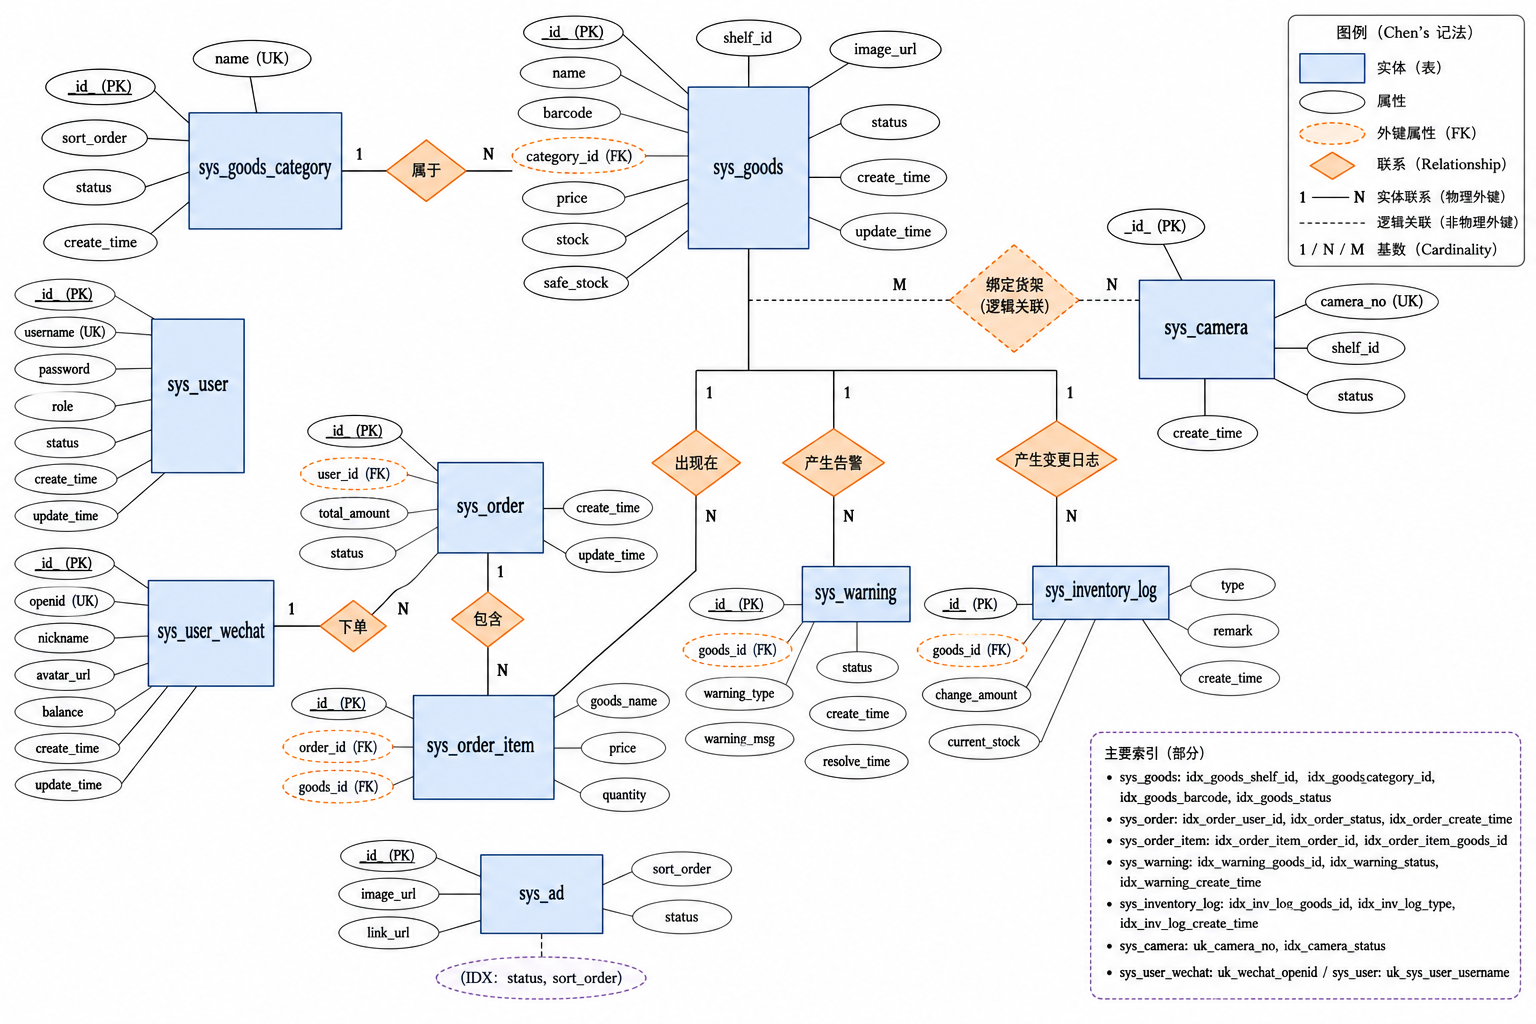
\includegraphics[width=0.95\textwidth]{images/fig-er-diagram.png}\\[0.3em]
  {\zihao{-5}图4-1\quad 系统概念数据库设计——ER 图}
\end{center}

系统数据库 \texttt{retail\_db} 共包含 10 个实体，核心实体及联系描述如下：

\begin{itemize}[leftmargin=2em]
  \item \textbf{系统用户（sys\_user）}与\textbf{订单（sys\_order）}：一对多关系，一个管理端用户可创建多个订单。
  \item \textbf{小程序用户（sys\_user\_wechat）}与\textbf{订单（sys\_order）}：一对多关系，一个小程序用户可创建多个订单。
  \item \textbf{订单（sys\_order）}与\textbf{订单明细（sys\_order\_item）}：一对多关系，一个订单包含多条明细。
  \item \textbf{商品（sys\_goods）}与\textbf{订单明细（sys\_order\_item）}：一对多关系，一个商品可出现在多条订单明细中。
  \item \textbf{商品分类（sys\_goods\_category）}与\textbf{商品（sys\_goods）}：一对多关系，一个分类下可有多个商品。
  \item \textbf{商品（sys\_goods）}与\textbf{库存告警（sys\_warning）}：一对多关系，一个商品可触发多条告警记录。
  \item \textbf{商品（sys\_goods）}与\textbf{库存变更日志（sys\_inventory\_log）}：一对多关系，一个商品有多条库存变更流水。
  \item \textbf{摄像头（sys\_camera）}与\textbf{商品（sys\_goods）}：通过 \texttt{shelf\_id} 字段逻辑关联，一个摄像头监控一个货架，一个货架上可摆放多个商品。
  \item \textbf{首页广告（sys\_ad）}：独立实体，与其他实体无外键关联。
\end{itemize}

\subsection{逻辑数据库设计}

以下按表逐一列出数据库 \texttt{retail\_db} 的全部 10 张表的逻辑结构。

\paragraph{1. 系统用户表（sys\_user）}
\begin{center}
  \renewcommand{\arraystretch}{1.4}
  \zihao{5}
  \begin{tabular}{|>{\centering\arraybackslash}m{2.5cm}|>{\centering\arraybackslash}m{3.2cm}|>{\centering\arraybackslash}m{4.4cm}|>{\centering\arraybackslash}m{3.5cm}|}
    \hline
    \textbf{字段名} & \textbf{数据类型}   & \textbf{约束}    & \textbf{说明}        \\ \hline
    id           & BIGINT UNSIGNED & PK, 自增         & 主键 ID              \\ \hline
    username     & VARCHAR(64)     & NOT NULL, UK   & 用户名                \\ \hline
    password     & VARCHAR(255)    & NOT NULL       & 密码                 \\ \hline
    role         & ENUM            & NOT NULL       & 角色（admin/customer） \\ \hline
    status       & TINYINT         & NOT NULL, 默认 1 & 状态（1 启用/0 禁用）      \\ \hline
    create\_time & DATETIME        & NOT NULL       & 创建时间               \\ \hline
    update\_time & DATETIME        & NOT NULL       & 更新时间（自动维护）         \\ \hline
  \end{tabular}
  \\[0.3em]
  {\zihao{-5}表4-1\quad sys\_user 表结构}
\end{center}

\paragraph{2. 商品分类表（sys\_goods\_category）}
\begin{center}
  \renewcommand{\arraystretch}{1.4}
  \zihao{5}
  \begin{tabular}{|>{\centering\arraybackslash}m{2.5cm}|>{\centering\arraybackslash}m{3.2cm}|>{\centering\arraybackslash}m{4.4cm}|>{\centering\arraybackslash}m{3.5cm}|}
    \hline
    \textbf{字段名} & \textbf{数据类型}   & \textbf{约束}    & \textbf{说明} \\ \hline
    id           & BIGINT UNSIGNED & PK, 自增         & 分类 ID       \\ \hline
    name         & VARCHAR(64)     & NOT NULL, UK   & 分类名称        \\ \hline
    sort\_order  & INT             & NOT NULL, 默认 0 & 排序值         \\ \hline
    status       & TINYINT         & NOT NULL, 默认 1 & 状态          \\ \hline
    create\_time & DATETIME        & NOT NULL       & 创建时间        \\ \hline
  \end{tabular}
  \\[0.3em]
  {\zihao{-5}表4-2\quad sys\_goods\_category 表结构}
\end{center}

\paragraph{3. 商品基础表（sys\_goods）}
\begin{center}
  \renewcommand{\arraystretch}{1.4}
  \zihao{5}
  \begin{tabular}{|>{\centering\arraybackslash}m{2.5cm}|>{\centering\arraybackslash}m{3.2cm}|>{\centering\arraybackslash}m{4.4cm}|>{\centering\arraybackslash}m{3.5cm}|}
    \hline
    \textbf{字段名} & \textbf{数据类型}   & \textbf{约束}     & \textbf{说明} \\ \hline
    id           & BIGINT UNSIGNED & PK, 自增          & 主键 ID       \\ \hline
    name         & VARCHAR(128)    & NOT NULL        & 商品名称        \\ \hline
    barcode      & VARCHAR(64)     & 可空, 索引          & 条形码         \\ \hline
    category\_id & BIGINT UNSIGNED & 可空, 索引          & 分类 ID       \\ \hline
    price        & DECIMAL(10,2)   & NOT NULL        & 商品价格        \\ \hline
    stock        & INT             & NOT NULL, 默认 0  & 库存数量        \\ \hline
    safe\_stock  & INT             & NOT NULL, 默认 10 & 安全库存阈值      \\ \hline
    shelf\_id    & VARCHAR(64)     & NOT NULL, 索引    & 货架编号        \\ \hline
    image\_url   & VARCHAR(255)    & 可空              & 商品图片 URL    \\ \hline
    status       & TINYINT         & NOT NULL, 默认 1  & 上/下架状态      \\ \hline
    create\_time & DATETIME        & NOT NULL        & 创建时间        \\ \hline
    update\_time & DATETIME        & NOT NULL        & 更新时间        \\ \hline
  \end{tabular}
  \\[0.3em]
  {\zihao{-5}表4-3\quad sys\_goods 表结构}
\end{center}

\paragraph{4. 订单主表（sys\_order）}
\begin{center}
  \renewcommand{\arraystretch}{1.4}
  \zihao{5}
  \begin{tabular}{|>{\centering\arraybackslash}m{2.5cm}|>{\centering\arraybackslash}m{3.2cm}|>{\centering\arraybackslash}m{4.4cm}|>{\centering\arraybackslash}m{3.5cm}|}
    \hline
    \textbf{字段名}  & \textbf{数据类型}   & \textbf{约束}  & \textbf{说明} \\ \hline
    id            & BIGINT UNSIGNED & PK, 自增       & 订单 ID       \\ \hline
    user\_id      & BIGINT UNSIGNED & NOT NULL, 索引 & 用户 ID       \\ \hline
    total\_amount & DECIMAL(10,2)   & NOT NULL     & 订单总金额       \\ \hline
    status        & VARCHAR(32)     & NOT NULL     & 订单状态        \\ \hline
    create\_time  & DATETIME        & NOT NULL, 索引 & 创建时间        \\ \hline
    update\_time  & DATETIME        & NOT NULL     & 更新时间        \\ \hline
  \end{tabular}
  \\[0.3em]
  {\zihao{-5}表4-4\quad sys\_order 表结构}
\end{center}

\paragraph{5. 订单明细表（sys\_order\_item）}
\begin{center}
  \renewcommand{\arraystretch}{1.4}
  \zihao{5}
  \begin{tabular}{|>{\centering\arraybackslash}m{2.5cm}|>{\centering\arraybackslash}m{3.2cm}|>{\centering\arraybackslash}m{4.4cm}|>{\centering\arraybackslash}m{3.5cm}|}
    \hline
    \textbf{字段名} & \textbf{数据类型}   & \textbf{约束}    & \textbf{说明} \\ \hline
    id           & BIGINT UNSIGNED & PK, 自增         & 明细 ID       \\ \hline
    order\_id    & BIGINT UNSIGNED & NOT NULL, 索引   & 订单 ID       \\ \hline
    goods\_id    & BIGINT UNSIGNED & NOT NULL, 索引   & 商品 ID       \\ \hline
    goods\_name  & VARCHAR(128)    & NOT NULL       & 商品名称快照      \\ \hline
    price        & DECIMAL(10,2)   & NOT NULL       & 商品单价快照      \\ \hline
    quantity     & INT             & NOT NULL, 默认 1 & 购买数量        \\ \hline
  \end{tabular}
  \\[0.3em]
  {\zihao{-5}表4-5\quad sys\_order\_item 表结构}
\end{center}

\paragraph{6. 库存告警表（sys\_warning）}
\begin{center}
  \renewcommand{\arraystretch}{1.4}
  \zihao{5}
  \begin{tabular}{|>{\centering\arraybackslash}m{2.5cm}|>{\centering\arraybackslash}m{3.2cm}|>{\centering\arraybackslash}m{4.4cm}|>{\centering\arraybackslash}m{3.5cm}|}
    \hline
    \textbf{字段名}  & \textbf{数据类型}   & \textbf{约束}    & \textbf{说明} \\ \hline
    id            & BIGINT UNSIGNED & PK, 自增         & 告警 ID       \\ \hline
    goods\_id     & BIGINT UNSIGNED & NOT NULL, 索引   & 商品 ID       \\ \hline
    warning\_type & VARCHAR(32)     & NOT NULL       & 告警类型        \\ \hline
    warning\_msg  & VARCHAR(255)    & NOT NULL       & 告警内容        \\ \hline
    status        & TINYINT         & NOT NULL, 默认 0 & 处理状态        \\ \hline
    create\_time  & DATETIME        & NOT NULL, 索引   & 创建时间        \\ \hline
    resolve\_time & DATETIME        & 可空             & 处理时间        \\ \hline
  \end{tabular}
  \\[0.3em]
  {\zihao{-5}表4-6\quad sys\_warning 表结构}
\end{center}

\paragraph{7. 库存变更日志表（sys\_inventory\_log）}
\begin{center}
  \renewcommand{\arraystretch}{1.4}
  \zihao{5}
  \begin{tabular}{|>{\centering\arraybackslash}m{2.5cm}|>{\centering\arraybackslash}m{3.2cm}|>{\centering\arraybackslash}m{4.4cm}|>{\centering\arraybackslash}m{3.5cm}|}
    \hline
    \textbf{字段名}   & \textbf{数据类型}   & \textbf{约束}  & \textbf{说明} \\ \hline
    id             & BIGINT UNSIGNED & PK, 自增       & 日志 ID       \\ \hline
    goods\_id      & BIGINT UNSIGNED & NOT NULL, 索引 & 商品 ID       \\ \hline
    change\_amount & INT             & NOT NULL     & 变动数量（正/负）   \\ \hline
    current\_stock & INT             & NOT NULL     & 变动后当前库存     \\ \hline
    type           & VARCHAR(32)     & NOT NULL, 索引 & 日志类型        \\ \hline
    remark         & VARCHAR(255)    & 可空           & 备注          \\ \hline
    create\_time   & DATETIME        & NOT NULL, 索引 & 创建时间        \\ \hline
  \end{tabular}
  \\[0.3em]
  {\zihao{-5}表4-7\quad sys\_inventory\_log 表结构}
\end{center}

\paragraph{8. 小程序用户表（sys\_user\_wechat）}
\begin{center}
  \renewcommand{\arraystretch}{1.4}
  \zihao{5}
  \begin{tabular}{|>{\centering\arraybackslash}m{2.5cm}|>{\centering\arraybackslash}m{3.2cm}|>{\centering\arraybackslash}m{4.4cm}|>{\centering\arraybackslash}m{3.5cm}|}
    \hline
    \textbf{字段名} & \textbf{数据类型}   & \textbf{约束}    & \textbf{说明} \\ \hline
    id           & BIGINT UNSIGNED & PK, 自增         & 主键 ID       \\ \hline
    openid       & VARCHAR(128)    & NOT NULL, UK   & 微信用户唯一标识    \\ \hline
    nickname     & VARCHAR(64)     & 可空             & 昵称          \\ \hline
    avatar\_url  & VARCHAR(255)    & 可空             & 头像 URL      \\ \hline
    balance      & DECIMAL(10,2)   & NOT NULL, 默认 0 & 钱包余额        \\ \hline
    create\_time & DATETIME        & NOT NULL       & 创建时间        \\ \hline
    update\_time & DATETIME        & NOT NULL       & 更新时间        \\ \hline
  \end{tabular}
  \\[0.3em]
  {\zihao{-5}表4-8\quad sys\_user\_wechat 表结构}
\end{center}

\paragraph{9. 首页轮播广告表（sys\_ad）}
\begin{center}
  \renewcommand{\arraystretch}{1.4}
  \zihao{5}
  \begin{tabular}{|>{\centering\arraybackslash}m{2.5cm}|>{\centering\arraybackslash}m{3.2cm}|>{\centering\arraybackslash}m{4.4cm}|>{\centering\arraybackslash}m{3.5cm}|}
    \hline
    \textbf{字段名} & \textbf{数据类型}   & \textbf{约束}    & \textbf{说明} \\ \hline
    id           & BIGINT UNSIGNED & PK, 自增         & 主键 ID       \\ \hline
    image\_url   & VARCHAR(255)    & NOT NULL       & 轮播图 URL     \\ \hline
    link\_url    & VARCHAR(255)    & 可空             & 点击跳转链接      \\ \hline
    sort\_order  & INT             & NOT NULL, 默认 0 & 排序值         \\ \hline
    status       & TINYINT         & NOT NULL, 默认 1 & 启用状态        \\ \hline
  \end{tabular}
  \\[0.3em]
  {\zihao{-5}表4-9\quad sys\_ad 表结构}
\end{center}

\paragraph{10. 摄像头管理表（sys\_camera）}
\begin{center}
  \renewcommand{\arraystretch}{1.4}
  \zihao{5}
  \begin{tabular}{|>{\centering\arraybackslash}m{2.5cm}|>{\centering\arraybackslash}m{3.2cm}|>{\centering\arraybackslash}m{4.4cm}|>{\centering\arraybackslash}m{3.5cm}|}
    \hline
    \textbf{字段名} & \textbf{数据类型}   & \textbf{约束}    & \textbf{说明}   \\ \hline
    id           & BIGINT UNSIGNED & PK, 自增         & 摄像头 ID        \\ \hline
    camera\_no   & VARCHAR(32)     & NOT NULL, UK   & 摄像头编号         \\ \hline
    shelf\_id    & VARCHAR(64)     & NOT NULL       & 绑定货架编号        \\ \hline
    status       & TINYINT         & NOT NULL, 默认 1 & 状态（1 正常/0 停用） \\ \hline
    last\_scan\_time & DATETIME    & 可空             & 最近一次巡检时间      \\ \hline
    create\_time & DATETIME        & NOT NULL       & 创建时间          \\ \hline
  \end{tabular}
  \\[0.3em]
  {\zihao{-5}表4-10\quad sys\_camera 表结构}
\end{center}

%%% ==================== 5 系统出错处理设计 ==================== %%%
\section{系统出错处理设计}

\subsection{出错信息}

系统通过 GlobalExceptionHandler（\texttt{@RestControllerAdvice}）统一拦截所有异常，将其转换为标准 Result 结构返回，避免堆栈信息直接暴露给前端。以下为系统可能出现的出错信息一览表：

\begin{center}
  \renewcommand{\arraystretch}{1.4}
  \zihao{5}
  \begin{tabular}{|>{\centering\arraybackslash}m{1.5cm}|>{\centering\arraybackslash}m{4.8cm}|>{\centering\arraybackslash}m{5.5cm}|}
    \hline
    \textbf{业务码} & \textbf{触发场景}    & \textbf{提示信息}                           \\ \hline
    400          & 请求参数缺失或非法        & “商品 ID 不能为空”“分页参数必须大于 0”等               \\ \hline
    400          & 请求体 JSON 格式错误    & “请求体 JSON 格式错误”                         \\ \hline
    400          & camera\_no 已被绑定  & “该 camera\_no 已被绑定”                     \\ \hline
    400          & 小程序登录 code 非法    & “演示环境仅支持 code=test\_code”               \\ \hline
    401          & 未登录或 Token 过期/无效 & “未登录或Token无效”                           \\ \hline
    404          & 资源不存在            & “商品不存在或修改失败”“摄像头不存在”“告警不存在”             \\ \hline
    404          & 接口路径错误           & “接口不存在，请检查请求路径”                         \\ \hline
    405          & 请求方法不匹配          & “请求方法不支持”                               \\ \hline
    415          & Content-Type 不支持 & “Content-Type 不支持，请使用 application/json” \\ \hline
    500          & 数据库操作失败          & “新增商品失败”“处理告警失败”等                       \\ \hline
    500          & 摄像头预览数据为空        & “摄像头预览数据为空”                             \\ \hline
    500          & 未知系统异常           & “服务器内部异常”                               \\ \hline
    502          & Python AI 服务调用失败 & “调用 Python XX 服务失败”                     \\ \hline
  \end{tabular}
  \\[0.3em]
  {\zihao{-5}表5-1\quad 系统出错信息一览}
\end{center}

前端出错提示设计：
\begin{itemize}[leftmargin=2em]
  \item 管理端（retail-admin-pro）：通过 Axios 拦截器统一捕获非 200 响应，调用 \texttt{checkStatus} 函数根据 HTTP 状态码映射为 Element Plus 的 ElMessage 弹窗提示；403/404/500 等页面级错误显示专用错误页面。
  \item 小程序端（retail-customer）：在 \texttt{wx.request} 的 fail 回调和 success 中判断 \texttt{res.data.code}，非 200 时通过 \texttt{wx.showToast} 显示友好错误提示。
\end{itemize}

\subsection{补救措施}

\begin{enumerate}[leftmargin=2em]
  \item \textbf{JWT 令牌过期}：前端拦截 401 响应后自动清除本地 Token 并跳转登录页面，要求用户重新认证。管理端通过 Axios 拦截器实现，小程序端在请求封装层判断后调用 \texttt{wx.redirectTo} 跳转至登录页。
  \item \textbf{AI 服务宕机}：retail-server 对所有 RestTemplate 调用进行 try-catch 包裹，捕获 RestClientException 后返回 502 错误码。AI 服务不可用不影响商品管理、购物车、订单结算等核心功能的正常运行。
  \item \textbf{数据库事务失败}：订单结算（checkout）在 Service 层使用数据库事务，库存扣减与订单写入在同一事务中执行。若任一步骤失败，事务自动回滚，保证不出现“钱已扣但库存未减”的数据不一致。
  \item \textbf{摄像头资源泄露}：retail-ai 的 CameraManager 采用引用计数机制，每次 acquire 增加计数、release 减少计数。后台 Reaper 线程每 5 秒扫描一次，对引用计数归零且空闲超过 60 秒的摄像头自动执行硬件释放。服务关闭时 \texttt{on\_shutdown} 钩子释放所有摄像头。
  \item \textbf{Redis 缓存不可用}：推荐流接口在 Redis 无数据时返回 204（无更多数据），不影响用户使用其他功能。购物车使用 Redis 存储时，异常降级为返回空列表。
  \item \textbf{并发请求冲突}：商品库存更新通过 MyBatis-Plus 的条件更新保证数据安全；摄像头管理器内部使用 \texttt{threading.Lock} 保证线程安全。
  \item \textbf{文件上传失败}：FileController 校验上传文件大小和类型，异常时返回明确错误信息，不会导致服务崩溃。
  \item \textbf{网络中断}：前端均设置请求超时（管理端 Axios 超时配置、小程序 wx.request timeout），超时后显示“网络异常”提示，用户可手动重试。
\end{enumerate}

\swjtuChapter{系统详细设计报告}

% 去掉章节前缀，使用 1 / 1.1 / 1.1.1 的编号体系
\setcounter{section}{0}
\renewcommand{\thesection}{\arabic{section}}
\renewcommand{\thesubsection}{\thesection.\arabic{subsection}}
\renewcommand{\thesubsubsection}{\thesubsection.\arabic{subsubsection}}

\section{引言}

\subsection{编写目的}
本文档在《软件需求规格说明书》和《系统概要设计报告》的基础上，对系统核心模块进行部件级细化设计，明确前后端交互、类与接口职责、关键业务时序及异常处理策略，为编码实现、联调测试和后期运维提供统一依据。

\subsection{项目背景}
“零售物品智能识别系统”面向商超场景，目标是打通顾客侧“搜索/识别/下单”链路与管理侧“商品维护/库存预警/摄像头巡检”链路。当前项目由四个子系统组成：
\begin{itemize}[leftmargin=2em]
  \item \textbf{retail-admin-pro}：管理端前端（Vue3 + Vite）。
  \item \textbf{retail-customer}：微信小程序客户端。
  \item \textbf{retail-server}：Spring Boot 后端服务，负责业务编排与数据一致性。
  \item \textbf{retail-ai}：FastAPI AI 服务，提供摄像头、识别、搜索能力。
\end{itemize}

\subsection{参考文献}
\begin{enumerate}[leftmargin=2em]
  \item 《软件工程：实践者的研究方法》
  \item Spring Boot 3.3 官方文档
  \item FastAPI 官方文档
  \item 微信小程序开发文档
  \item MyBatis-Plus 官方文档
\end{enumerate}

\section{系统功能需求概要}

系统按业务闭环划分为三个主模块：
\begin{enumerate}[leftmargin=2em]
  \item \textbf{智能视觉导购模块}：支持文本检索、图片识别、货架定位。
  \item \textbf{交易与结算模块}：支持购物车管理、库存校验、订单生成、支付确认。
  \item \textbf{后台商品与库存监控模块}：支持商品维护、摄像头管理、告警处理、定时巡检。
\end{enumerate}

模块间关系如下：
\begin{itemize}[leftmargin=2em]
  \item 顾客侧通过小程序与后端交互，后端按需转发 AI 能力调用。
  \item 管理员侧通过管理端维护主数据与调度参数。
  \item 交易成功后触发库存与告警联动，低库存时由后台机制继续触发补给流程。
\end{itemize}

\begin{center}
  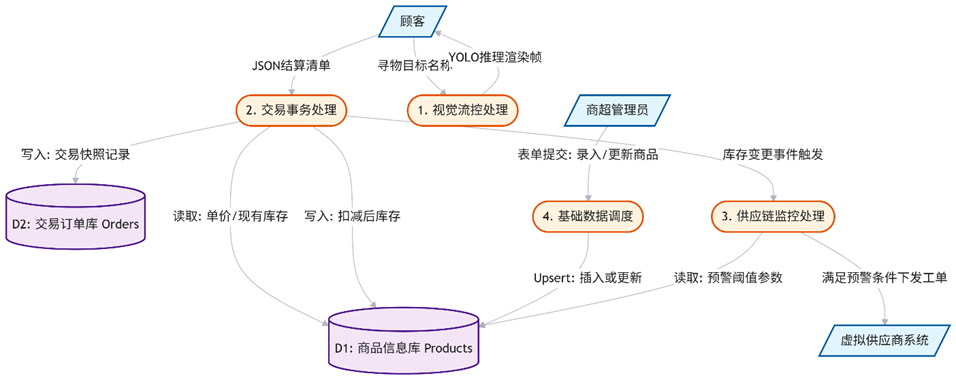
\includegraphics[width=0.9\textwidth]{images/图3-9.png}\\[0.3em]
  {\zihao{-5}图3-1\quad 系统一层数据流（用于功能分解映射）}
\end{center}

\section{智能视觉导购模块详细设计}

\subsection{功能模块概述}
智能视觉导购模块聚焦"找得到、看得见、加得进购物车"，主要功能为：
\begin{itemize}[leftmargin=2em]
  \item 文本检索：小程序调用 \texttt{GET /api/goods/page} 通过名称模糊搜索与分类筛选查找商品。
  \item 图片识别：小程序上传 base64 图像至 \texttt{POST /api/applet/scan}，后端调用 \texttt{POST /api/ai/recognize/center} 返回去重后的 Top-K 商品候选。识别请求具备重试机制——后端最多重试 2 次（间隔 1s/2s），前端也支持最多 2 次自动重试，保障网络波动下的可用性。
  \item 商品详情补全：通过 \texttt{POST /api/applet/goods/listByIds} 将识别出的 ID 列表转换为可展示的商品信息。
\end{itemize}

\subsection{用户交互界面设计}
顾客端对应页面与交互如下：
\begin{enumerate}[leftmargin=2em]
  \item \textbf{查询页（pages/search）}：输入关键词，实时节流检索，展示结果与推荐流。点击"加入购物车"按钮直接添加 1 件商品到购物车（无需二次确认），展开 +/- 数量控件后增减操作自动同步购物车，数量减至 0 时自动移出购物车。
  \item \textbf{识别页（pages/scan）}：拍照或相册选图后，发起识别并在页面展示去重后的候选商品。识别接口支持前后端双重重试机制，确保弱网环境下的成功率。识别结果按商品类别去重，避免同一商品重复展示。
  \item \textbf{商品详情页（pages/goods）}：查看单品信息并加入购物车。
\end{enumerate}

交互设计原则：
\begin{itemize}[leftmargin=2em]
  \item 请求期间给出加载态，避免重复点击。
  \item 识别失败自动重试，最终失败时提示友好错误信息。
  \item 商品加入购物车后即时反馈，并更新购物车角标；加减购操作直接同步后端，无需额外确认步骤。
\end{itemize}

\subsection{类及接口细化设计}

\subsubsection{核心类与职责}
\begin{itemize}[leftmargin=2em]
  \item \texttt{AppletCameraController}：接收 \texttt{image\_base64}，调用 AI 聚合服务。
  \item \texttt{AppletGoodsController}：按 ID 批量查询商品详情。
  \item \texttt{GoodsController}：提供商品分页检索（按名称模糊搜索 + 分类筛选 + 价格排序）。
  \item \texttt{AiIntegrationServiceImpl}：统一封装与 Python AI 的 HTTP 调用，内置去重逻辑与最多 2 次自动重试。
  \item \texttt{recognition/routes.py}：实现中心点识别（按类别去重）与批量货架识别。
\end{itemize}

\subsubsection{关键接口说明}
\begin{center}
  \renewcommand{\arraystretch}{1.35}
  \zihao{5}
  \begin{tabular}{|>{\centering\arraybackslash}m{3.6cm}|>{\centering\arraybackslash}m{2.2cm}|>{\centering\arraybackslash}m{6.4cm}|}
    \hline
    \textbf{接口} & \textbf{方法} & \textbf{说明} \\ \hline
    /api/goods/page & GET & 商品分页检索，参数 \texttt{name}、\texttt{categoryId}、\texttt{page}、\texttt{size} \\ \hline
    /api/applet/scan & POST & 图片识别，参数 \texttt{image\_base64}、\texttt{k} \\ \hline
    /api/applet/goods/listByIds & POST & 按商品 ID 列表批量查询详情 \\ \hline
    /api/ai/recognize/center & POST & AI 中心点识别（内部接口，已去重） \\ \hline
  \end{tabular}
  \\[0.3em]
  {\zihao{-5}表3-1\quad 视觉导购模块关键接口}
\end{center}

\subsubsection{时序细化（文字时序）}
识别寻物主流程的时序如下：
\begin{enumerate}[leftmargin=2em]
  \item 顾客在小程序选择图片并提交。
  \item 小程序调用 \texttt{POST /api/applet/scan}，前端内置最多 2 次失败自动重试。
  \item 后端调用 AI 服务 \texttt{POST /api/ai/recognize/center} 获取候选 ID（Python 侧已按类别去重），后端内置最多 2 次重试。
  \item Python YOLO 检测器返回距画面中心最近的 k 个不同类别商品的坐标与置信度。
  \item 后端在结果组装阶段执行冗余去重校验，确保无重复商品。
  \item 后端查询商品主数据并补全名称、价格、库存、货架号。
  \item 后端返回候选列表；前端展示并支持加减购操作。
\end{enumerate}

\section{交易与结算模块详细设计}

\subsection{功能模块概述}
交易与结算模块负责购物车数据管理、订单结算、库存扣减及订单查询。关键约束为“库存扣减与订单写入必须同事务提交，失败则整体回滚”。

\subsection{用户交互界面设计}
顾客端交互主要在以下页面完成：
\begin{itemize}[leftmargin=2em]
  \item \textbf{购物车页（pages/cart）}：增减数量、勾选商品、清空购物车、进入结算。
  \item \textbf{订单页（pages/order）}：确认结算、查看历史订单、按状态筛选。
  \item \textbf{支付页（pages/payment）}：余额/微信支付方式选择与支付确认。
\end{itemize}

界面状态设计：
\begin{enumerate}[leftmargin=2em]
  \item 购物车为空时禁止结算。
  \item 结算中使用按钮锁定和 Loading，防止重复提交。
  \item 支付成功后跳转用户中心并刷新订单状态。
\end{enumerate}

\subsection{类及接口细化设计}

\subsubsection{核心类与职责}
\begin{itemize}[leftmargin=2em]
  \item \texttt{CartController} + \texttt{CartServiceImpl}：维护 Redis 购物车。
  \item \texttt{OrderController} + \texttt{OrderServiceImpl}：执行结算事务与订单查询。
  \item \texttt{GoodsMapper}：提供 \texttt{selectByIdForUpdate} 与 \texttt{decreaseStock} 原子扣减能力。
  \item \texttt{OrderItemMapper}、\texttt{InventoryLogMapper}：写入明细与库存流水。
\end{itemize}

\subsubsection{结算流程关键逻辑}
\begin{enumerate}[leftmargin=2em]
  \item 从 Redis 读取用户购物车并校验合法性。
  \item 对商品 ID 排序后逐条加锁（\texttt{FOR UPDATE}）降低并发死锁概率。
  \item 校验库存并执行条件扣减（\texttt{stock >= quantity}）。
  \item 写入库存日志，低于阈值时生成库存告警。
  \item 写入订单主表与订单明细表。
  \item 事务提交后异步清空 Redis 购物车。
\end{enumerate}

\subsubsection{关键接口说明}
\begin{center}
  \renewcommand{\arraystretch}{1.35}
  \zihao{5}
  \begin{tabular}{|>{\centering\arraybackslash}m{3.6cm}|>{\centering\arraybackslash}m{2.2cm}|>{\centering\arraybackslash}m{6.4cm}|}
    \hline
    \textbf{接口} & \textbf{方法} & \textbf{说明} \\ \hline
    /api/cart/add & POST & 加入/修改购物车商品数量 \\ \hline
    /api/cart/list & GET & 查询当前用户购物车 \\ \hline
    /api/order/checkout & POST & 管理端/通用结算接口 \\ \hline
    /api/applet/order/checkout & POST & 小程序结算接口（可携带清单） \\ \hline
    /api/applet/order/pay & POST & 小程序订单支付确认 \\ \hline
    /api/order/list & GET & 查询订单历史 \\ \hline
  \end{tabular}
  \\[0.3em]
  {\zihao{-5}表3-2\quad 交易与结算模块关键接口}
\end{center}

\section{后台商品与库存监控模块详细设计}

\subsection{功能模块概述}
该模块面向管理员与系统后台任务，完成商品全生命周期管理、库存告警治理、摄像头绑定与巡检调度。核心能力包括：
\begin{itemize}[leftmargin=2em]
  \item 商品分页查询、新增、编辑、删除、图片上传。
  \item 告警分页查询、告警处理、未处理告警聚合。
  \item 摄像头绑定、预览、流式代理、调度参数动态更新。
  \item 定时巡检调用 AI 批量识别并同步货架商品信息。
\end{itemize}

\subsection{用户交互界面设计}
管理端对应页面如下：
\begin{enumerate}[leftmargin=2em]
  \item \textbf{商品管理页（views/goods/manage）}：搜索、增删改、库存可视标签、图片上传。
  \item \textbf{视觉调度页（views/camera/schedule）}：摄像头绑定、预览、巡检配置、手动触发。
  \item \textbf{数据看板页（views/dashboard/dataVisualize）}：展示销售、库存和告警概览。
\end{enumerate}

\subsection{类及接口细化设计}

\subsubsection{核心类与职责}
\begin{itemize}[leftmargin=2em]
  \item \texttt{GoodsController}：商品 CRUD 与库存补货日志触发。
  \item \texttt{WarningController} / \texttt{AdminWarningController}：告警分页与待处理清单。
  \item \texttt{CameraController}：摄像头管理与流代理接口。
  \item \texttt{CameraScanScheduler}：定时任务调度、分批调用 AI、同步货架信息。
  \item \texttt{GlobalExceptionHandler}：统一异常转换与错误码输出。
\end{itemize}

\subsubsection{调度时序细化（文字时序）}
\begin{enumerate}[leftmargin=2em]
  \item 定时器按 \texttt{interval-minutes} 触发巡检任务。
  \item 读取状态正常的摄像头列表并按 \texttt{batch-size} 分批。
  \item 后端向 \texttt{/api/ai/recognize/shelf/batch} 提交批量识别请求。
  \item 收到 \texttt{detected\_goods\_ids} 后回写商品 \texttt{shelf\_id}。
  \item 输出巡检日志，供管理员在页面和日志系统中查看。
\end{enumerate}

\subsubsection{关键接口说明}
\begin{center}
  \renewcommand{\arraystretch}{1.35}
  \zihao{5}
  \begin{tabular}{|>{\centering\arraybackslash}m{3.6cm}|>{\centering\arraybackslash}m{2.2cm}|>{\centering\arraybackslash}m{6.4cm}|}
    \hline
    \textbf{接口} & \textbf{方法} & \textbf{说明} \\ \hline
    /api/goods/page & GET & 商品分页查询 \\ \hline
    /api/goods & POST/PUT & 商品新增与编辑 \\ \hline
    /api/warning/page & GET & 告警分页查询 \\ \hline
    /api/warning/\{id\}/resolve & PUT & 告警处理 \\ \hline
    /api/admin/camera/list & GET & 摄像头列表 \\ \hline
    /api/admin/camera/scheduler/config & GET/PUT & 巡检参数查询与更新 \\ \hline
    /api/admin/camera/scheduler/trigger & POST & 手动触发巡检 \\ \hline
  \end{tabular}
  \\[0.3em]
  {\zihao{-5}表3-3\quad 后台监控模块关键接口}
\end{center}

本章从模块职责、界面交互、类与接口、关键时序四个层面完成了详细设计，后续测试用例与部署方案均以本章为实现依据。

\swjtuChapter{系统测试报告}

% 去掉章节前缀，使用 1 / 1.1 / 1.1.1 的编号体系
\setcounter{section}{0}
\renewcommand{\thesection}{\arabic{section}}
\renewcommand{\thesubsection}{\thesection.\arabic{subsection}}
\renewcommand{\thesubsubsection}{\thesubsection.\arabic{subsubsection}}

\section{项目简介}

\subsection{项目业务功能介绍}
系统业务覆盖“顾客购前导购、购中结算、购后库存联动”全链路，核心流程如下：
\begin{enumerate}[leftmargin=2em]
  \item 顾客通过小程序进行文本检索或图片识别，定位目标商品。
  \item 顾客将商品加入购物车并发起结算。
  \item 后端校验库存并生成订单，写入库存日志与告警信息。
  \item 管理员在管理端维护商品与摄像头，并通过巡检调度监控货架状态。
\end{enumerate}

\begin{center}
  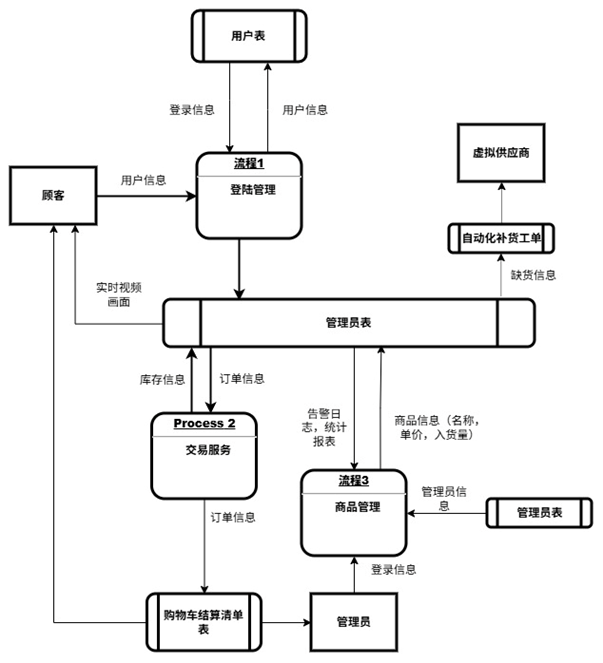
\includegraphics[width=0.9\textwidth]{images/图3-8.png}\\[0.3em]
  {\zihao{-5}图4-1\quad 系统顶层数据流（测试对象边界）}
\end{center}

\subsection{术语及主要名称介绍}
\begin{itemize}[leftmargin=2em]
  \item \textbf{白盒测试}：基于代码逻辑路径的测试方法，关注语句、条件、路径覆盖。
  \item \textbf{黑盒测试}：基于需求输入输出的测试方法，关注功能行为与边界。
  \item \textbf{冒烟测试}：以最小用例集合快速验证核心流程可用性。
  \item \textbf{基线路径}：选取系统中最关键、最高频的业务路径进行持续回归。
\end{itemize}

\subsection{参考文献}
\begin{enumerate}[leftmargin=2em]
  \item 《软件测试的艺术》
  \item ISTQB 基础级测试标准
  \item Postman 官方文档
  \item JMeter 官方文档
\end{enumerate}

\section{测试需求说明}

\subsection{编写目的}
本文档用于明确测试范围、测试策略、测试环境与验收标准，确保系统交付前在功能正确性、稳定性与可维护性方面满足课程项目要求。

\subsection{系统功能需求}
本轮测试覆盖以下功能域：
\begin{itemize}[leftmargin=2em]
  \item 登录鉴权（管理端与小程序）。
  \item 商品管理（分页、增删改、图片上传）。
  \item 购物车与订单结算（加购、结算、订单查询、支付）。
  \item 库存告警（生成、分页查询、处理）。
  \item 摄像头与巡检调度（绑定、预览、手动触发、参数更新）。
  \item AI 接口联动（文本检索、中心识别、批量识别）。
\end{itemize}

\subsection{非功能性需求指标}
\begin{center}
  \renewcommand{\arraystretch}{1.35}
  \zihao{5}
  \begin{tabular}{|>{\centering\arraybackslash}m{2.8cm}|>{\centering\arraybackslash}m{4.0cm}|>{\centering\arraybackslash}m{5.4cm}|}
    \hline
    \textbf{指标类别} & \textbf{目标值} & \textbf{说明} \\ \hline
    接口响应 & 常规接口 P95 \textless= 200ms & 在本地联调网络下，剔除图片上传与视频流场景 \\ \hline
    识别能力 & 单帧推理时延可控、结果稳定返回 & 重点验证接口可用性与字段完整性 \\ \hline
    一致性 & 订单与库存同事务提交 & 失败时必须回滚，避免脏数据 \\ \hline
    可恢复性 & 异常时返回统一错误结构 & 全局异常处理器输出 \texttt{code/message/data} \\ \hline
  \end{tabular}
  \\[0.3em]
  {\zihao{-5}表4-1\quad 非功能性测试指标}
\end{center}

\subsection{环境需求}
\begin{itemize}[leftmargin=2em]
  \item 操作系统：Windows 10/11。
  \item JDK：21。
  \item Maven：3.9+。
  \item Python：3.10+，依赖 \texttt{fastapi/uvicorn/opencv-python/numpy/pydantic}。
  \item Node.js：18+（项目当前环境为 Node.js 24）。
  \item 数据库与缓存：MySQL 8.x、Redis 8.x。
  \item 客户端工具：Postman、微信开发者工具。
\end{itemize}

\subsection{测试人员要求}
\begin{enumerate}[leftmargin=2em]
  \item 熟悉 RESTful 接口测试、HTTP 状态码与 JSON 结构校验。
  \item 能阅读 Java/Python 关键业务代码，完成白盒路径分析。
  \item 能使用 Postman/JMeter 执行功能与性能测试。
\end{enumerate}

\subsection{测试标准}
\begin{itemize}[leftmargin=2em]
  \item 关键业务链路（登录、加购、结算、告警）必须通过。
  \item 高风险缺陷（导致数据错误或流程中断）必须关闭。
  \item 非阻断类问题可带条件上线，但需有规避方案与修复计划。
\end{itemize}

\section{测试计划}

本次测试采用“先冒烟后回归”的策略：
\begin{enumerate}[leftmargin=2em]
  \item \textbf{阶段一：接口冒烟测试}，验证主流程可跑通。
  \item \textbf{阶段二：白盒路径覆盖}，针对结算、鉴权、巡检等核心代码进行路径分析和用例补齐。
  \item \textbf{阶段三：黑盒方法测试}，按等价类、边界值、判定表、场景法执行回归。
  \item \textbf{阶段四：性能与异常测试}，验证可用性与容错性。
\end{enumerate}

入口条件：后端、AI、数据库、缓存服务已启动；初始化数据已导入。  
退出条件：主流程缺陷清零，回归用例通过率满足验收要求。

\section{测试过程及用例}

\subsection{白盒测试用例}
白盒测试聚焦 \texttt{OrderServiceImpl.checkout}、\texttt{JwtAuthInterceptor.preHandle}、\texttt{CameraScanScheduler.executeScanBatchTask} 三条关键链路。

\subsubsection{语句覆盖}
\begin{center}
  \renewcommand{\arraystretch}{1.35}
  \zihao{5}
  \begin{tabular}{|>{\centering\arraybackslash}m{1.8cm}|>{\centering\arraybackslash}m{4.0cm}|>{\centering\arraybackslash}m{5.8cm}|}
    \hline
    \textbf{用例ID} & \textbf{测试目标} & \textbf{预期结果} \\ \hline
    WB-S-01 & 用户未登录直接结算 & 返回 401，流程中止 \\ \hline
    WB-S-02 & 购物车为空结算 & 返回 400，提示购物车为空 \\ \hline
    WB-S-03 & 库存充足正常结算 & 生成订单、写入明细、库存扣减成功 \\ \hline
    WB-S-04 & AI 批量识别调用异常 & 返回 502，调度任务记录错误日志 \\ \hline
  \end{tabular}
  \\[0.3em]
  {\zihao{-5}表4-2\quad 白盒语句覆盖用例}
\end{center}

\subsubsection{条件覆盖}
\begin{itemize}[leftmargin=2em]
  \item 条件 C1：\texttt{userId == null || userId < 1}
  \item 条件 C2：\texttt{goods.stock < quantity}
  \item 条件 C3：\texttt{remainStock < 10}
\end{itemize}

对应条件覆盖用例如下：
\begin{center}
  \renewcommand{\arraystretch}{1.35}
  \zihao{5}
  \begin{tabular}{|>{\centering\arraybackslash}m{1.8cm}|>{\centering\arraybackslash}m{3.3cm}|>{\centering\arraybackslash}m{3.0cm}|>{\centering\arraybackslash}m{3.5cm}|}
    \hline
    \textbf{用例ID} & \textbf{输入场景} & \textbf{覆盖条件} & \textbf{预期结果} \\ \hline
    WB-C-01 & 无 Token 请求 & C1=True & 返回 401 \\ \hline
    WB-C-02 & 库存不足下单 & C2=True & 事务回滚，返回库存不足 \\ \hline
    WB-C-03 & 库存临界值下单 & C3=True & 订单成功且生成告警 \\ \hline
    WB-C-04 & 库存充足下单 & C1/C2/C3=False & 订单成功，无告警 \\ \hline
  \end{tabular}
  \\[0.3em]
  {\zihao{-5}表4-3\quad 白盒条件覆盖用例}
\end{center}

\subsubsection{基本路径覆盖}
以结算模块构建控制流图后选取 4 条基本路径：
\begin{enumerate}[leftmargin=2em]
  \item P1：未登录路径（入口即失败）。
  \item P2：购物车为空路径（参数通过但业务拦截）。
  \item P3：库存不足路径（中途失败并回滚）。
  \item P4：成功路径（订单与库存均提交，异步清空购物车）。
\end{enumerate}

\subsection{黑盒测试用例}

\subsubsection{等价类划分}
\begin{center}
  \renewcommand{\arraystretch}{1.35}
  \zihao{5}
  \begin{tabular}{|>{\centering\arraybackslash}m{2.2cm}|>{\centering\arraybackslash}m{3.2cm}|>{\centering\arraybackslash}m{4.6cm}|>{\centering\arraybackslash}m{3.2cm}|}
    \hline
    \textbf{功能} & \textbf{有效等价类} & \textbf{无效等价类} & \textbf{判定} \\ \hline
    登录 & username/password 非空且匹配 & 用户名空、密码空、账号不存在、密码错误 & 返回 200/401/400 \\ \hline
    文本检索 & keyword 非空，k\textgreater=1 & keyword 为空，k\textless1 & 返回商品列表或 400 \\ \hline
    商品新增 & name/price/stock/shelfId 合法 & 关键字段缺失或类型非法 & 返回 200 或 400 \\ \hline
  \end{tabular}
  \\[0.3em]
  {\zihao{-5}表4-4\quad 黑盒等价类设计}
\end{center}

\subsubsection{边界值测试}
边界值选取：\texttt{page=1}、\texttt{size=1}、\texttt{k=1}、\texttt{k=100}、\texttt{stock=0}。  
预期：边界内可处理，越界返回参数错误或空结果。

\subsubsection{判定表法}
以“是否允许结算”为例构建判定表：
\begin{itemize}[leftmargin=2em]
  \item 条件：已登录 / 购物车非空 / 库存充足。
  \item 动作：允许结算并生成订单 / 拒绝并给出原因。
\end{itemize}

规则结论：仅当三个条件同时满足时执行结算；任一条件不满足均返回失败。

\subsubsection{因果图法}
因：低库存触发阈值（库存 \textless 安全库存）  
果：生成告警记录，并在管理端待处理列表可见。  
验证点：告警类型、消息文本、状态字段是否正确。

\subsubsection{场景法}
端到端场景 S1：
\begin{enumerate}[leftmargin=2em]
  \item 小程序登录。
  \item 文本检索商品并加入购物车。
  \item 发起结算并支付。
  \item 管理端查看订单与告警变化。
\end{enumerate}

S1 预期：订单生成成功；库存扣减；低库存商品触发告警。

\subsubsection{正交实验法}
针对“搜索体验”选取三因素进行组合：
\begin{itemize}[leftmargin=2em]
  \item 因素 A：搜索方式（文本/图片）。
  \item 因素 B：返回数量 k（3/10/20）。
  \item 因素 C：网络状态（正常/弱网）。
\end{itemize}

通过正交组合验证搜索稳定性与可用性，减少全排列测试成本。

\subsection{性能测试}

本轮性能测试采用“轻量压测 + 接口基准”方式：
\begin{itemize}[leftmargin=2em]
  \item 工具：Postman Runner（基准）、JMeter（并发脚本）。
  \item 对象：\texttt{/api/goods/page}、\texttt{/api/order/checkout}、\texttt{/api/applet/search/text}。
  \item 指标：平均响应时间、P95、错误率。
\end{itemize}

阶段性结论：当前版本已完成单用户和小并发基准验证，系统无阻断性错误；大并发压测建议在独立性能环境继续执行。

\subsection{其他测试}
\begin{itemize}[leftmargin=2em]
  \item \textbf{异常测试}：非法 JSON、错误 Content-Type、未授权 Token。
  \item \textbf{兼容性测试}：管理端 Chrome 浏览器、小程序开发者工具。
  \item \textbf{恢复测试}：AI 服务不可用、Redis 不可用时的降级与报错行为。
  \item \textbf{安全测试}：鉴权拦截、越权访问、敏感错误信息屏蔽。
\end{itemize}

\section{测试报告及分析}

\subsection{测试报告}
基于本阶段用例执行与联调记录，可得结论：
\begin{enumerate}[leftmargin=2em]
  \item 核心业务链路（登录、检索、加购、结算、告警）可闭环运行。
  \item 后端统一异常处理机制有效，错误返回结构一致。
  \item 事务型结算逻辑能够在库存不足场景下回滚，避免数据不一致。
\end{enumerate}

\subsection{缺陷报告}
\begin{center}
  \renewcommand{\arraystretch}{1.35}
  \zihao{5}
  \begin{tabular}{|>{\centering\arraybackslash}m{1.6cm}|>{\centering\arraybackslash}m{4.8cm}|>{\centering\arraybackslash}m{2.5cm}|>{\centering\arraybackslash}m{3.0cm}|}
    \hline
    \textbf{编号} & \textbf{缺陷描述} & \textbf{严重级别} & \textbf{状态} \\ \hline
    BUG-01 & 管理中心点识别返回结果未去重，同一商品被 YOLO 多次检测后在前端重复展示，导致加减购操作出现数量不一致 & 高 & 已修复 \\ \hline
    BUG-02 & AI 识别接口在并发或模型冷启动时偶发超时（原读取超时仅 10 秒），表现为"识别失败请重试" & 高 & 已修复 \\ \hline
    BUG-03 & 小程序查询页增减购操作无法将物品数量减至 0，且每次加入购物车需二次确认后才生效 & 中 & 已修复 \\ \hline
    BUG-04 & 登录页"我们的服务"区域 car 与 search 图标引用路径后缀为 .jpg，而实际文件为 .png，导致图标无法加载显示 & 低 & 已修复 \\ \hline
    BUG-05 & 小程序登录演示环境固定 \texttt{test\_code}，未接入真实 \texttt{code2Session} & 中 & 已知限制 \\ \hline
    BUG-06 & 管理员密码采用 BCrypt 加密存储，历史明文密码已通过自动迁移机制升级 & 低 & 已修复 \\ \hline
  \end{tabular}
  \\[0.3em]
  {\zihao{-5}表4-5\quad 主要缺陷汇总}
\end{center}

\subsection{分析总结}
\begin{itemize}[leftmargin=2em]
  \item 系统在课程项目目标范围内具备可交付性，功能链路完整。已修复的 4 项缺陷覆盖了识别去重、AI 服务容错、前端交互体验和资源加载四个维度。
  \item 当前主要风险集中于"生产级安全与工程化能力"（如微信真实登录对接），不影响课程演示，但需在后续版本中处理。
  \item 识别链路已实现 Python 侧与 Java 侧双端去重 + 前后端双重试机制，可靠性显著提升。
  \item 下一阶段建议补齐自动化测试（JUnit + 前端 E2E）与专项性能压测报告，提升回归效率与可信度。
\end{itemize}

\swjtuChapter{系统安装部署手册}

% 去掉章节前缀，使用 1 / 1.1 / 1.1.1 的编号体系
\setcounter{section}{0}
\renewcommand{\thesection}{\arabic{section}}
\renewcommand{\thesubsection}{\thesection.\arabic{subsection}}
\renewcommand{\thesubsubsection}{\thesubsection.\arabic{subsubsection}}

\section{编写目的}
本文档用于指导项目成员或实施人员在 Windows 环境完成系统部署，确保前后端、AI 服务、数据库与缓存服务能够按统一流程快速搭建并联调验证。

\subsection{读者对象}
\begin{itemize}[leftmargin=2em]
  \item 项目实施工程师
  \item 系统运维人员
  \item 课程验收与演示准备人员
\end{itemize}

\subsection{参考资料}
\begin{enumerate}[leftmargin=2em]
  \item Spring Boot 官方文档
  \item FastAPI 官方文档
  \item 微信小程序开发者工具文档
  \item 项目数据库脚本：\texttt{retail/retail\_db.sql}
\end{enumerate}

\section{安装部署要求}

\subsection{服务器要求}
\begin{center}
  \renewcommand{\arraystretch}{1.35}
  \zihao{5}
  \begin{tabular}{|>{\centering\arraybackslash}m{2.8cm}|>{\centering\arraybackslash}m{4.2cm}|>{\centering\arraybackslash}m{5.2cm}|}
    \hline
    \textbf{类型} & \textbf{最低配置} & \textbf{推荐配置} \\ \hline
    CPU & 4 核 & 8 核及以上 \\ \hline
    内存 & 8GB & 16GB 及以上 \\ \hline
    磁盘 & 20GB 可用空间 & 50GB SSD 可用空间 \\ \hline
    网络 & 千兆局域网 & 千兆局域网/专线 \\ \hline
    外设 & USB 摄像头（可选） & 高清摄像头 + 稳定光照 \\ \hline
  \end{tabular}
  \\[0.3em]
  {\zihao{-5}表5-1\quad 服务器硬件要求}
\end{center}

\subsection{支撑软件安装要求}
\begin{center}
  \renewcommand{\arraystretch}{1.35}
  \zihao{5}
  \begin{tabular}{|>{\centering\arraybackslash}m{2.8cm}|>{\centering\arraybackslash}m{2.8cm}|>{\centering\arraybackslash}m{6.4cm}|}
    \hline
    \textbf{软件} & \textbf{版本} & \textbf{说明} \\ \hline
    JDK & 21 & 运行 \texttt{retail-server} \\ \hline
    Maven & 3.9+ & 构建与启动 Spring Boot \\ \hline
    Python & 3.10+ & 运行 \texttt{retail-ai} \\ \hline
    Node.js & 18+ & 构建/运行 \texttt{retail-admin-pro} \\ \hline
    pnpm & 8+ & 前端依赖管理 \\ \hline
    MySQL & 8.x & 业务数据库 \texttt{retail\_db} \\ \hline
    Redis & 8.x & 购物车存储、Token 缓存与推荐流缓存 \\ \hline
    微信开发者工具 & 最新版 & 运行 \texttt{retail-customer} \\ \hline
  \end{tabular}
  \\[0.3em]
  {\zihao{-5}表5-2\quad 支撑软件要求}
\end{center}

\subsection{应用软件部署要求}
\begin{itemize}[leftmargin=2em]
  \item 开放端口：\texttt{5173}（管理端开发）、\texttt{8080}（后端）、\texttt{8000}（AI）、\texttt{3306}（MySQL）、\texttt{6379}（Redis）。
  \item 修改后端配置文件 \texttt{retail-server/src/main/resources/application.yml} 中数据库账号密码。
  \item 确保日志目录可写；默认日志路径为 \texttt{E:/retail/log/retail-server.log}，如不存在请提前创建或调整配置。
\end{itemize}

\section{部署方案}

\subsection{环境部署}

\subsubsection{步骤一：数据库初始化}
\begin{enumerate}[leftmargin=2em]
  \item 创建并初始化业务库：
  \begin{itemize}[leftmargin=2em]
    \item 执行脚本：\texttt{retail/retail\_db.sql}
    \item 可选测试数据：\texttt{mock\_data.sql}
  \end{itemize}
  \item 默认管理员账号：\texttt{admin}，默认密码：\texttt{123456}。
\end{enumerate}

\subsubsection{步骤二：Redis 启动}
可使用项目内置 Redis 目录启动（Windows）：
\begin{itemize}[leftmargin=2em]
  \item 启动脚本：\texttt{Redis-8.6.2-Windows-x64-msys2/Redis-8.6.2-Windows-x64-msys2/start.bat}
\end{itemize}

\subsubsection{步骤三：AI 服务部署（retail-ai）}
\begin{enumerate}[leftmargin=2em]
  \item 进入目录：\texttt{retail/retail-ai}
  \item 创建虚拟环境并安装依赖：\texttt{python -m venv .venv}，\texttt{pip install -r requirements.txt}
  \item 启动服务：\texttt{python main.py}
  \item 启动成功后默认监听：\texttt{http://localhost:8000}
\end{enumerate}

\subsubsection{步骤四：后端服务部署（retail-server）}
\begin{enumerate}[leftmargin=2em]
  \item 进入目录：\texttt{retail/retail-server}
  \item 执行启动命令：\texttt{mvn spring-boot:run}
  \item 若系统未安装 Maven，可使用项目内 Maven：\texttt{../../apache-maven-3.9.14/bin/mvn.cmd spring-boot:run}
  \item 启动后访问：\texttt{http://localhost:8080}
\end{enumerate}

\subsubsection{步骤五：管理端部署（retail-admin-pro）}
\begin{enumerate}[leftmargin=2em]
  \item 进入目录：\texttt{retail/retail-admin-pro}
  \item 安装依赖：\texttt{pnpm install}
  \item 启动开发服务：\texttt{pnpm dev}
  \item 访问地址：\texttt{http://localhost:5173}
\end{enumerate}

\subsubsection{步骤六：小程序端部署（retail-customer）}
\begin{enumerate}[leftmargin=2em]
  \item 使用微信开发者工具导入目录：\texttt{retail/retail-customer}
  \item 检查 \texttt{project.config.json} 的 \texttt{appid} 配置。
  \item 检查 \texttt{app.js} 与 \texttt{utils/request.js} 中后端地址（默认 \texttt{http://localhost:8080/api}）。
  \item 编译运行并验证登录、搜索、结算流程。
\end{enumerate}

\subsection{系统部署}

\subsubsection{部署拓扑}
系统采用“前端 + 后端 + AI + 数据库 + 缓存”分层部署：
\begin{itemize}[leftmargin=2em]
  \item 管理端通过 Vite 代理访问后端 \texttt{/api}。
  \item 小程序端通过 \texttt{wx.request} 访问后端 \texttt{/api/applet/*}。
  \item 后端通过 HTTP 调用 AI 服务 \texttt{/api/ai/*}。
  \item 后端通过 JDBC 访问 MySQL，通过 Lettuce 访问 Redis。
\end{itemize}

\subsubsection{部署验证清单}
建议按以下顺序验证：
\begin{enumerate}[leftmargin=2em]
  \item 访问 \texttt{http://localhost:8080/api/auth/login} 登录接口返回正常。
  \item 管理端可登录并进入“商品管理”页面。
  \item 管理端可查看“视觉调度”并触发一次巡检。
  \item 小程序可登录并完成“搜索-加购-结算”流程。
  \item 数据库中 \texttt{sys\_order}、\texttt{sys\_order\_item} 有新增记录。
\end{enumerate}

\subsubsection{常见故障与处理}
\begin{itemize}[leftmargin=2em]
  \item \textbf{后端启动失败（数据库连接）}：检查 \texttt{application.yml} 的 \texttt{datasource} 配置与 MySQL 服务状态。
  \item \textbf{管理端接口 401}：检查是否携带 Token，确认登录后本地缓存是否写入。
  \item \textbf{AI 调用 502}：检查 \texttt{retail-ai} 是否在 8000 端口运行。
  \item \textbf{摄像头不可用}：检查摄像头权限、设备占用状态及 DirectShow 驱动。
\end{itemize}

\swjtuChapter{系统用户操作手册}

% 去掉章节前缀，使用 1 / 1.1 / 1.1.1 的编号体系
\setcounter{section}{0}
\renewcommand{\thesection}{\arabic{section}}
\renewcommand{\thesubsection}{\thesection.\arabic{subsection}}
\renewcommand{\thesubsubsection}{\thesubsection.\arabic{subsubsection}}

\section{商超管理员角色操作手册}

\subsection{登录功能使用说明}
\begin{enumerate}[leftmargin=2em]
  \item 在浏览器访问管理端首页（默认：\texttt{http://localhost:5173}）。
  \item 输入管理员账号与密码（默认 \texttt{admin/123456}）。
  \item 点击"登录"进入系统首页。
\end{enumerate}

异常提示：若提示"未登录或 Token 无效"，请重新登录并确认后端服务正常运行。

\subsection{商品管理功能使用说明}
进入菜单"商品管理"后，可进行以下操作：
\begin{enumerate}[leftmargin=2em]
  \item \textbf{查询商品}：输入商品名称关键字，点击"搜索"。
  \item \textbf{新增商品}：点击"新增商品"，填写名称、价格、库存、货架号并上传图片后提交。
  \item \textbf{编辑商品}：点击列表"编辑"按钮更新商品信息。
  \item \textbf{删除商品}：点击"删除"并确认。
\end{enumerate}

操作结果：系统通过接口 \texttt{/api/goods}、\texttt{/api/upload} 返回成功消息，列表自动刷新。

\subsection{视觉调度功能使用说明}
进入菜单"视觉调度"后，可进行以下操作：
\begin{enumerate}[leftmargin=2em]
  \item \textbf{新增摄像头绑定}：选择物理摄像头索引并填写货架号。
  \item \textbf{编辑绑定关系}：修改指定摄像头对应货架号。
  \item \textbf{删除摄像头}：移除无效或停用设备。
  \item \textbf{更新巡检参数}：设置巡检间隔（分钟）和分批大小（台）。
  \item \textbf{手动触发巡检}：点击按钮立即执行一次全量扫描。
\end{enumerate}

建议：修改巡检参数后观察日志，确认任务已按新参数重启。

\subsection{告警与看板功能使用说明}
\begin{enumerate}[leftmargin=2em]
  \item 在告警列表中查看未处理库存预警。
  \item 对已确认问题执行"处理告警"操作。
  \item 在数据看板查看销售趋势、库存健康度与近期告警概览。
\end{enumerate}

\section{顾客角色操作手册}

\subsection{登录功能使用说明}
\begin{enumerate}[leftmargin=2em]
  \item 打开小程序进入"我的"页面。
  \item 点击"登录"，授权微信用户信息。
  \item 登录成功后，系统在本地保存 Token 与用户资料。
\end{enumerate}

说明：演示环境中小程序登录使用固定测试码 \texttt{test\_code}。

\subsection{查询功能使用说明}
\begin{enumerate}[leftmargin=2em]
  \item 进入"查询"页输入关键词，系统自动节流检索并展示结果。
  \item 在筛选栏可按分类、价格区间和价格排序进一步缩小范围。
  \item 点击商品可查看详情，或点击"加入购物车"按钮直接添加 1 件商品至购物车（无需二次确认）。
  \item 展开的 +/- 数量控件可直接调整数量，增减操作自动同步至购物车，数量减至 0 时该商品自动移出购物车。
\end{enumerate}

提示：若返回"未找到相关商品"，可尝试更换关键词或使用图片识别。

\subsection{视觉识别寻物功能使用说明}
\begin{enumerate}[leftmargin=2em]
  \item 进入"识别"页，选择"拍照"或"从相册选择"。
  \item 系统上传图片并执行 AI 识别（内置自动重试机制，弱网环境下更稳定）。
  \item 识别结果去重展示商品名称、价格、置信度与货架编号，通过 +/- 按钮调整数量后直接同步购物车。
\end{enumerate}

异常处理：若多次重试后仍提示"识别失败"，请稍后重试或检查 AI 服务运行状态。

\subsection{购物车与结算功能使用说明}
\begin{enumerate}[leftmargin=2em]
  \item 在"购物车"页勾选商品并调整数量。
  \item 点击"去结算"进入订单确认页。
  \item 确认金额后提交结算，系统生成订单号。
\end{enumerate}

结算规则：库存不足时系统会阻止下单，并提示库存异常信息。

\subsection{订单、支付与充值功能使用说明}
\begin{enumerate}[leftmargin=2em]
  \item 在"我的-订单"中查看历史订单与状态。
  \item 对待付款订单进入支付页，选择余额或微信方式。
  \item 余额不足时可进入充值页完成账户充值。
\end{enumerate}

\section{系统后台角色操作手册}

\subsection{巡检任务运行说明}
系统后台内置摄像头巡检任务，默认每 5 分钟执行一次：
\begin{itemize}[leftmargin=2em]
  \item 读取状态正常的摄像头列表。
  \item 分批调用 AI 批量识别接口。
  \item 同步识别到的商品与货架关系。
  \item 记录任务日志并返回结果。
\end{itemize}

\subsection{参数调整与手动触发说明}
运维人员可在管理端"视觉调度"页面完成：
\begin{enumerate}[leftmargin=2em]
  \item 调整巡检间隔与批次大小。
  \item 手动触发全量巡检，用于快速复核库存陈列。
\end{enumerate}

\subsection{异常处理说明}
\begin{itemize}[leftmargin=2em]
  \item \textbf{AI 服务不可达}：后端返回 502，建议先恢复 \texttt{retail-ai} 后重试。AI 识别接口已内置自动重试机制，短暂恢复后可自动重连成功。
  \item \textbf{数据库异常}：结算流程自动回滚，避免脏数据。
  \item \textbf{摄像头占用}：释放视频流资源后重新预览。
  \item \textbf{Token 过期}：前端清理登录态并引导重新登录。
\end{itemize}

\subsection{运维建议}
\begin{enumerate}[leftmargin=2em]
  \item 每日检查 \texttt{retail-server.log} 和巡检任务日志。
  \item 每周备份 MySQL 业务库和关键配置文件。
  \item 定期清理无效摄像头绑定与历史无效告警。
  \item 监控 AI 服务响应延迟，及时调整识别超时与重试参数。
\end{enumerate}


%%% ===================== 结致参附 ===================== %%%
%%% ----------------------- 结论 ----------------------- %%%
% \include{chapters/conclusion}

%%% ----------------------- 致谢 ----------------------- %%%
% \include{chapters/acknowledgments}

%%% --------------------- 参考文献 --------------------- %%%
\swjtuBibliography{参考文献}

%%% ----------------------- 附录 ----------------------- %%%
% \include{appendix/appendix1}
% \include{appendix/appendix2}

\end{document}
